\documentclass[10pt,oneside]{book}

\input{utils/packages}

\makeindex

\newcommand{\minitab}[2][l]{\begin{tabular}{@{}#1@{}}#2\end{tabular}}


\definecolor{ListingBG}{rgb}{0.91,0.91,0.91}
\definecolor{shadecolor}{rgb}{0.92,0.92,0.92}

\hyphenation{Open-SHMEM}

\renewcommand{\chaptername}{Chapter}
\renewcommand{\appendixname}{Annex}
\Crefname{appendix}{Annex}{Annexes}

% Place some penalty for doing the break
\def\gb{\penalty10000\hskip 0pt plus 8em\penalty4800\hskip 0pt plus-8em%
\penalty10000}

% Searchable underscore with allowed line break after it
\DeclareRobustCommand{\_}{\texttt{\char`\_}\discretionary{}{}{}}

\def\colorswapnt{\colorlet{saved}{.}\color{ForestGreen}}
\def\colorswapot{\colorlet{saved}{.}\color{red}}
\def\prevcolor{\color{saved}}

\newcommand{\newtext}[1]{\textcolor{ForestGreen}{#1}}
\newcommand{\oldtext}[1]{\textcolor{magenta}{\sout{#1}}}
\newcommand{\insertDocVersion}{0.1}
\newcommand{\openshmem}[1][]{%
  {Open\-SHMEM\ifthenelse{\equal{#1}{}}{}{~#1}}\xspace}
\newcommand{\HEADER}[1]{\textit{#1}}
\newcommand{\FUNC}[1]{\textit{#1}}
\newcommand{\CTYPE}[1]{\textit{#1}}
\newcommand{\VAR}[1]{\textit{#1}}
\newcommand{\ENVVAR}[1]{\textit{#1}}
\newcommand{\CONST}[1]{\textit{#1}}
\newcommand{\KEYWORD}[1]{\textit{#1}}
%%
\newcommand{\CorCpp}{\textit{C/C++}\xspace}
\newcommand{\Cstd}[1][]{%
  \textit{C\ifthenelse{\equal{#1}{}}{}{#1}}\xspace}
%%
\newcommand{\TYPE}{\emph{TYPE}}
\newcommand{\TYPENAME}{\emph{TYPENAME}}
\newcommand{\SIZE}{\emph{SIZE}}

\newcommand{\source}{\textit{source}}
\newcommand{\dest}{\textit{dest}}
\newcommand{\PUT}{\textit{Put}}
\newcommand{\GET}{\textit{Get}}
\newcommand{\OPR}[1]{\textit{#1}}
\newcommand{\shmemprefix}{\textit{SHMEM\_}}
\newcommand{\shmemprefixLC}{\textit{shmem\_}}
\newcommand{\shmemgprefix}{\textit{shmemg\_}}
\newcommand{\ith}{${\textit{i}^{\text{\tiny th}}}$}
\newcommand{\jth}{${\textit{j}^{\text{\tiny th}}}$}

%% Generate indexed reference.
\newcommand{\EnvVarIndex}[1]{\index{#1}}
\newcommand{\FuncIndex}[1]{\index{#1}}
\newcommand{\LibConstIndex}[1]{\index{#1}}
\newcommand{\LibHandleIndex}[1]{\index{#1}}
\newcommand{\TableIndex}[1]{\index{#1}\index{Tables!#1}}
%% Write text and generate reference.
\newcommand{\EnvVarRef}[1]{\ENVVAR{#1}\EnvVarIndex{#1}}
\newcommand{\FuncRef}[1]{\FUNC{#1}\FuncIndex{#1}}
\newcommand{\LibConstRef}[1]{\CONST{#1}\LibConstIndex{#1}}
\newcommand{\LibHandleRef}[1]{\CONST{#1}\LibHandleIndex{#1}}
\newcommand{\TableCaptionRef}[1]{\caption{#1}\TableIndex{#1}}
%% Specialized declaration/creation and generate reference.
\newcommand{\EnvVarDecl}[1]{\EnvVarRef{#1}}
\newcommand{\FuncDecl}[1]{{\ListingsCurrentStyle{#1}}\FuncIndex{#1}}
\newcommand{\FuncParam}[1]{{\ListingsParamStyle{#1}}}
\newcommand{\LibConstDecl}[2][\CorCpp]{%
  \parbox[t]{5cm}{~\\[-4pt] #1: \\\hspace*{8mm} \LibConstRef{#2} \\~}}
\newcommand{\LibHandleDecl}[2][\CorCpp]{%
  \parbox[t]{0pt}{~\\[-4pt] #1: \\\hspace*{8mm} \LibHandleRef{#2} \\~}}

\newcommand{\subsubsubsection}[1]{\paragraph{#1}\mbox{}\par\nobreak}
\Crefname{paragraph}{Section}{Sections}
\setlength{\parindent}{0pt}

\begin{acronym}
\acro{RMA}{Remote Memory Access}
\acro{RMO}{\emph{Remote Memory Operation}}
\acro{AMO}{Atomic Memory Operation}
\acro{PE}{\emph{Processing Element}}
\acrodefplural{PE}[PEs]{\emph{Processing Elements}}
\acro{PGAS}{\emph{Partitioned Global Address Space}}
\acro{API}{\emph{Application Programming Interface}}
\acro{GPU}{\emph{Graphics Processing Unit}}
\end{acronym}

% Remove whitespace and retain commas when using cleveref's `\cref`.
\makeatletter
\let\org@@cref\@cref
\renewcommand*{\@cref}[2]{%
  \edef\process@me{%
    \noexpand\org@@cref{#1}{\zap@space#2 \@empty}%
  }\process@me
}
\makeatother
\newcommand{\ChangelogRef}[1]{\\See \cref{#1}.\space}

% Grab current listings style for use in environment escape to LaTeX.
\makeatletter
\newcommand\ListingsCurrentStyle{}
\lst@AddToHook{Output}{\global\let\ListingsCurrentStyle\lst@thestyle}
\lst@AddToHook{OutputOther}{\global\let\ListingsCurrentStyle\lst@thestyle}
\makeatother

%
% Use Sans Serif font for sections
%
\makeatletter
\def\section{\@startsection {section}{1}{\z@}{-3.5ex plus -1ex minus
-.2ex}{2.3ex plus .2ex}{\Large\sf}}
\def\subsection{\@startsection{subsection}{2}{\z@}{-3.25ex plus -1ex minus
-.2ex}{1.5ex plus .2ex}{\large\sf}}
\def\subsubsection{\@startsection{subsubsection}{3}{\z@}{-3.25ex plus
-1ex minus -.2ex}{1.5ex plus .2ex}{\normalsize\sf\bf}}
\def\paragraph{\@startsection {paragraph}{4}{\z@}{3.25ex plus 1ex minus .2ex}
{-1em}{\normalsize\sf\bf}}
\makeatother

%
% Listings styles
%

\newcommand{\ListingsParamStyle}{\bfseries\itshape\color{CadetBlue}}

\definecolor{DarkGreen}{rgb}{0, 0.25, 0}

\lstdefinestyle{SourceListingsDefault}{
  language={C},
  breaklines=true,
  breakatwhitespace=true,
  escapechar=@,
  tabsize=2,
  basicstyle=\ttfamily\footnotesize,
  showstringspaces=false,
  frame=single,
  classoffset=0,
  keywords={\#include, \#pragma, \#if, \#ifdef, \#else, \#endif},
  keywordstyle=\bfseries\color{CadetBlue},
  classoffset=1,
  keywords={
    if, else, for, while, do, return, break, continue,
    static, const, volatile,
    sizeof, typedef, struct, union,
    switch, case, default, goto,
  },
  keywordstyle=\bfseries\color{Orchid},
  classoffset=2,
  keywords={
    __device__, _Thread_local, _Noreturn,
    void, bool, _Bool, unsigned, char, short, int, long,
    float, double, _Complex, complex, size_t, ptrdiff_t,
    int8_t, int16_t, int32_t, int64_t,
    uint8_t, uint16_t, uint32_t, uint64_t,
    shmem_ctx_t, shmem_team_t, shmem_team_config_t,
    FILE,
  },
  keywordstyle=\color{DarkGreen},
  classoffset=3,
  keywords={NULL},
  keywordstyle=\color{MidnightBlue},
  classoffset=4,
  keywords={TYPE, TYPENAME, SIZE},
  keywordstyle=\ListingsParamStyle,
  commentstyle=\itshape\color{BrickRed},
  stringstyle=\color{DarkOrchid},
  backgroundcolor=\color{white},
}

\definecolor{gray}{rgb}{0.97,0.97,0.97}

\lstdefinestyle{PrototypeListingsDefault}{
  style=SourceListingsDefault,
  frame=none,
  backgroundcolor=\color{gray},
}

\lstset{style=SourceListingsDefault}

%
% Library API description template commands
%

\newcommand{\apisummary}[1]{
    #1
\hfill
}

\newenvironment{apidefinition}{
\begin{description}
\item[SYNOPSIS] \hfill \\ \\
\vspace{-2em}
}
{
\end{description} % ends \begin{description} from \apidescription
\end{description}
}

\lstnewenvironment{Csynopsis}
{
  \textbf{C:}
  \lstset{style=PrototypeListingsDefault}
}{}

\lstnewenvironment{CsynopsisCol}
{
  \lstset{style=PrototypeListingsDefault}
}{}

\newenvironment{apiarguments}{
\newcommand{\apiargument}[3]{
\begin{tabular}{p{2cm} p{2cm} p{10cm}}
\textbf{##1} & \textit{##2} & {##3} \\
\end{tabular}
}
\hfill
\item[DESCRIPTION] \hfill

\begin{description}
\item[Arguments] \hfill \\
}
{
\hfill
\end{description}
}

\newcommand{\apidescription}[1]{
\begin{description}
\vspace{-1em}
\item[API Description] \hfill \\
    \sloppy
    #1
\hfill
}

\newcommand{\apireturnvalues}[1]{
\item[Return Values] \hfill \\
    #1
}

\newcommand{\apinotes}[1]{
\item[Notes] \hfill \\
    #1
}


\begin{document}

\hypersetup{pageanchor=true,citecolor=blue}

% Set header/footer for opening content
\pagestyle{fancy}
\fancyhead{}
\fancyhead[L]{\insertDocVersion}
\fancyhead[C]{--- DRAFT ---}
\SetWatermarkText{DRAFT}
\SetWatermarkScale{1}
\SetWatermarkLightness{.91}
\fancyfoot[C]{\thepage}

\pagenumbering{roman}

% Cover page
\thispagestyle{empty}
\begin{center}
\textbf{\Huge \openshmem}
\par
\end{center}

\begin{center}
\textbf{\LARGE Auxiliary Specification for GPU Support}\\
\vspace{1em}
\url{http://www.openshmem.org/}
\par
\end{center}

\begin{center}
Version \insertDocVersion
\par
\end{center}

\vspace{0.5in}
\begin{center}
Based on \openshmem 1.6
\end{center}

\vspace{0.5in}
\begin{center}
\today
\end{center}

\vfill{}

\pagebreak{}

\phantomsection
\section*{Authors and Collaborators}
\addcontentsline{toc}{section}{Authors and Collaborators}

The following individuals contributed to the development of this auxiliary
specification:

\begin{longtable}{p{0.42\textwidth}p{0.50\textwidth}}
\textbf{Name} & \textbf{Affiliation} \\
\hline
Johnathan Alsop & Advanced Micro Devices, Inc. \\
Michael Beebe & Texas Tech University \\
Aurelien Bouteiller & Advanced Micro Devices, Inc. \\
Mark F. Brown & Intel Corporation \\
Akihiro Hayashi & Georgia Institute of Technology \\
Oscar Hernandez & Oak Ridge National Laboratory \\
Avinash Kethineedi & Advanced Micro Devices, Inc. \\
Jeongnim Kim & Intel Corporation \\
Benjamin Michalowicz & The Ohio State University \\
Steve Poole & Los Alamos National Laboratory \\
Wendy Poole & Los Alamos National Laboratory \\
Brandon Potter & Advanced Micro Devices, Inc. \\
Md. Wasi-ur-Rahman & Hewlett Packard Enterprise (HPE) \\
Naveen Ravichandrasekaran & Hewlett Packard Enterprise (HPE) \\
Vivek Sarkar & Georgia Institute of Technology \\
Jun Shirako & Georgia Institute of Technology \\
Shubhendra Pal Singhal & Georgia Institute of Technology \\
Lawrence C. Stewart & Serissa Research \\
Thiago Teixeria & Intel Corporation \\
Y{\i}ltan Hassan Temu\c{c}in & Advanced Micro Devices, Inc. \\
Aaron Welch & Oak Ridge National Laboratory \\
Nathan Wichmann & Hewlett Packard Enterprise (HPE) \\
\end{longtable}

\pagebreak{}

\setcounter{tocdepth}{4}
\setcounter{secnumdepth}{4}
\tableofcontents

\mainmatter

% Set header/footer for main content
\pagestyle{fancy}
\fancyhf{}
\fancyhead[L]{\leftmark}
\fancyhead[R]{\thepage}
\renewcommand{\headrulewidth}{0pt}
\renewcommand{\thesection}{\arabic{section}}

\setlength{\parskip}{3pt}


% Section 1: Introduction

\section{Introduction}\label{sec:introduction}

\openshmem Auxiliary Specification for GPU Support defines extensions to the
\openshmem library interface specification for GPU-aware and GPU-centric
communication. These extensions allow \openshmem implementations to use
GPU-attached memory buffers for remote memory access, atomic memory operations,
and synchronization while maintaining compatibility with the core \openshmem
programming model.

Two communication paradigms are defined:

\begin{description}
\item[GPU-Aware Communication]
A programming model in which GPU-attached memory buffers may be used as source
or destination operands in \openshmem operations. The host \ac{PE} invokes
\openshmem routines, and the implementation shall manage data transfers
involving GPU-attached memory.

\item[GPU-Centric Communication]
A programming model in which communication operations may be initiated directly
from \ac{GPU} execution contexts, such as device kernels. \ac{GPU} threads invoke
\openshmem routines without host-side intervention.
\end{description}



% Section 2: Relationship to OpenSHMEM

\section{Relationship to OpenSHMEM}\label{sec:relationship}

The \openshmem Auxiliary Specification for GPU Support is based on the
\openshmem specification version 1.6. It supplements, but does not replace, the
\openshmem 1.6 specification. All routines, semantics, and requirements defined
in \openshmem 1.6 remain valid. Where new concepts are introduced or existing
semantics are modified, such changes are explicitly identified.

The extensions maintain the fundamental principles established by the \openshmem
specification, including:
\begin{itemize}
\item Processing elements (\acp{PE}) and symmetric data objects
\item Team-based process subsets and communication contexts
\item Memory ordering and synchronization guarantees
\item Collective and point-to-point communication semantics
\end{itemize}

Implementation of these extensions is optional. An \openshmem implementation may
support GPU-aware communication, GPU-centric communication, both, or neither.
Applications may query implementation capabilities at runtime.
Examples of GPU-aware and GPU-centric communication are provided in
\cref{annex:writing}.

Applications that do not use GPU-attached memory buffers or the interfaces
defined herein shall continue to execute correctly.



% Section 3: Specification Scope

\section{Specification Scope}\label{sec:scope}

The following are defined:
\begin{itemize}
\item Extensions to the \openshmem memory model to support a \ac{GPU} symmetric
  heap allocated from GPU-attached memory
\item Host-side interfaces for allocating and managing symmetric data objects
  within the \ac{GPU} symmetric heap
\item Device-side interfaces for initiating communication operations from
  \ac{GPU} execution contexts (\ac{GPU} kernels)
\item Semantics for data movement, atomic memory operations, and synchronization
  involving GPU-attached symmetric memory
\item Runtime capability reporting via \FUNC{shmem\_init\_thread}
\item Requirements for memory ordering and coherence when both the default and
  \ac{GPU} symmetric heaps are in use
\end{itemize}

The following are \textbf{not} defined:
\begin{itemize}
\item GPU programming models, device kernel languages, or GPU runtime APIs
\item Mechanisms for selecting or assigning GPUs to processing elements
\item Specific GPU architectures, vendor-specific features, or device driver
  interfaces
\item Performance characteristics, optimization requirements, or benchmarking
  methodologies
\item Network hardware capabilities, protocols, or transport-layer mechanisms
\item Extensions for non-GPU accelerators (FPGAs, DSPs, TPUs, DPUs, etc.)
\end{itemize}



% Section 4: Execution Model

\section{Execution Model}\label{sec:execution_model}

The execution model defined by the \openshmem specification is extended by the
introduction of a \ac{GPU} symmetric heap allocated from GPU-attached memory.
This \ac{GPU} symmetric heap is distinct from, and in addition to, the default
symmetric heap defined by the \openshmem specification.

\subsection{Processing Elements and GPU Association}\label{subsec:pe_gpu_association}

The concept of a processing element (\ac{PE}) is defined by the \openshmem
specification. In this version of the specification, every \ac{PE} in an
\openshmem program that uses the GPU support defined herein shall be associated
with exactly one \ac{GPU}. The association between a \ac{PE} and its \ac{GPU}
shall be established during initialization of the \openshmem library and shall
remain fixed for the duration of the program.

The mechanism by which a \ac{GPU} is selected for association with a \ac{PE} is
outside the scope of this specification. The application or runtime environment
shall select the \ac{GPU} prior to initialization of the \openshmem library. The
\openshmem implementation shall use the \ac{GPU} that has been made current or
otherwise designated by the execution environment at the time of library
initialization.

\subsection{GPU Symmetric Heap}\label{subsec:gpu_symmetric_heap}

The \ac{GPU} symmetric heap is distributed across \acp{PE}, with each \ac{PE}'s
allocation residing in the memory of its associated \ac{GPU}. Routines are
provided for allocating and managing the \ac{GPU} symmetric heap memory from the host,
and for performing one-sided read (get), write (put), atomic, signaling, and synchronization
operations on symmetric objects within it from both the host and \ac{GPU}
execution contexts. These routines follow the \ac{PGAS} programming model
established by the \openshmem specification.

\subsection{Memory Domains}\label{subsec:memory_domains}

Because symmetric data may reside in either host-attached or GPU-attached memory,
this specification distinguishes two \emph{memory domains}. A memory domain is
the address space with respect to which the ordering, completion, and atomicity
of \openshmem operations are defined. Each \ac{PE} that uses the GPU support
defined herein exposes two distinct memory domains:

\begin{description}
\item[Default memory domain] The default symmetric heap, together with the
symmetric static and global data objects defined by the \openshmem
specification, residing in host (CPU-attached) memory.
\item[\ac{GPU} memory domain] The \ac{GPU} symmetric heap, residing in the
device (GPU-attached) memory of the \ac{GPU} associated with the \ac{PE}
(\cref{subsec:pe_gpu_association}).
\end{description}

Private (non-symmetric) host or device memory belongs to neither memory domain
and cannot be the remote target of an \openshmem operation.

The two memory domains are independent. Operations issued to one memory domain
are neither ordered nor completed with respect to operations issued to the other
memory domain unless a completion routine such as \FUNC{shmem\_quiet} is called,
or unless a routine explicitly provides cross-domain ordering, such as the
put-with-signal routines. The corresponding ordering and completion rules are
defined in \cref{subsec:gpu_aware_ordering} for GPU-aware operations and in
\cref{subsec:gc_ordering} for GPU-centric operations.

\textbf{Interaction with teams and atomicity domains:} Memory ordering and
completion are tracked per memory domain and per communication context, while
atomicity is defined per atomicity domain (\cref{subsec:atomicity_domains}). The
predefined device teams \CONST{SHMEM\_DEVICE\_TEAM\_WORLD} and
\CONST{SHMEM\_DEVICE\_TEAM\_SHARED} form atomicity domains that are independent
of those rooted at the host teams \CONST{SHMEM\_TEAM\_WORLD} and
\CONST{SHMEM\_TEAM\_SHARED}. The team \CONST{SHMEM\_DEVICE\_TEAM\_SHARED}
identifies the \acp{PE} that share a \ac{GPU} memory domain and can therefore
directly load/store one another's \ac{GPU} symmetric heap objects
(\cref{subsec:shmem_device_team_shared}). A communication context created with
the \CONST{SHMEM\_DEVICE\_CTX} option operates on the \ac{GPU} memory domain;
a context created without that option operates on the default memory domain.

\textbf{Memory domains targeted by each operation type:} The following table
summarizes which memory domains may be named by the operands of each class of
operation.

\begin{longtable}{|p{4.6cm}|p{9.9cm}|}
\hline
\textbf{Operation type} & \textbf{Memory domains that may be targeted} \\
\hline
\endfirsthead
\hline
\textbf{Operation type} & \textbf{Memory domains that may be targeted} \\
\hline
\endhead
CPU / host-initiated (\openshmem 1.6) & Default memory domain only. \\
\hline
GPU-aware (\cref{sec:gpu_aware}) & Default memory domain and \ac{GPU} memory
domain; a single host-initiated routine may name operands in either domain. \\
\hline
GPU-centric (\cref{sec:gpu_centric}) & \ac{GPU} memory domain only; source,
destination, and synchronization operands shall reside in the \ac{GPU} symmetric
heap. \\
\hline
\end{longtable}



% Section 5: Communication Model

\section{Communication Model}\label{sec:communication_model}

The one-sided communication semantics defined by the \openshmem specification
apply to symmetric objects allocated from the \ac{GPU} symmetric heap. All
routines defined in \openshmem 1.6---including \ac{RMA}, \ac{AMO}, signaling,
synchronization, and collective operations---retain their specified behavior and
may be used with GPU-attached memory buffers.

The remote operand in a communication operation may reside in either the default
(CPU-attached) symmetric heap defined by \openshmem 1.6 or the \ac{GPU}
symmetric heap for the GPU-aware communication operations. For GPU-centric
communication operations, the remote operand shall reside in the \ac{GPU}
symmetric heap only. The same \openshmem routine shall be used regardless of whether
the remote memory is CPU-attached or GPU-attached.

\subsection{GPU-Aware Communication}\label{subsec:gpu_aware_comm}

GPU-aware communication allows GPU-attached memory buffers to be used as
operands in existing \openshmem routines without modification to interfaces or
calling conventions. GPU-attached memory buffers may be used as:

\begin{itemize}
\item \textbf{Source operands} in put operations
\item \textbf{Destination operands} in get operations
\item \textbf{Local operands} in atomic memory operations
\item \textbf{Target buffers} in point-to-point synchronization operations
\item \textbf{Local buffers} in collective operations
\end{itemize}

When a GPU-attached memory buffer is used as an operand in an \openshmem
routine, the \openshmem implementation shall make the contents of that buffer
available to the communication operation and shall make updates visible according
to the completion and ordering semantics defined in \openshmem 1.6. This
requirement does not prescribe the implementation mechanism, such as direct
network access to GPU-attached memory, staging through CPU-attached memory, or
runtime synchronization with the \ac{GPU} memory hierarchy.

\subsection{GPU-Centric Communication}\label{subsec:gpu_centric_comm}

GPU-centric communication allows \ac{GPU} threads to invoke put, get, atomic,
signaling, synchronization, and collective operations directly from \ac{GPU}
execution contexts. Device-initiated
operations use the same addressing model defined by the \openshmem
specification: a symmetric address and a target \ac{PE} identifier. The
symmetric address shall be within the allocated region returned by the \ac{GPU} symmetric heap
allocation routine and is valid only at the \ac{PE} where the allocation was
performed.

\textbf{Note:} Support for GPU-centric communication is independent of support
for GPU-aware communication; an implementation may support either or both.

\subsection{Supported Operations}\label{subsec:supported_operations}

The following operations are supported on symmetric objects in the \ac{GPU}
symmetric heap:

\begin{longtable}{|p{5cm}|p{9cm}|}
\hline
\textbf{Operation} & \textbf{Description} \\
\hline
\endfirsthead
\hline
\textbf{Operation} & \textbf{Description} \\
\hline
\endhead
\ac{RMA} & Put and get operations, including bulk and single-element variants \\
\hline
\ac{AMO} & Fetch, non-fetch, and compare-and-swap variants \\
\hline
Signaling Operations & Combined data transfer and signal update at the target \ac{PE} \\
\hline
Synchronization & Barrier, fence, quiet, and point-to-point wait/test primitives \\
\hline
\end{longtable}

\subsection{Ordering and Completion}\label{subsec:ordering_completion}

Ordering and completion semantics follow the \openshmem memory model. Updates to
symmetric objects are unordered by default. A \ac{PE} may enforce point-to-point
ordering using \FUNC{shmem\_fence}. \FUNC{shmem\_quiet} may be used to ensure
completion of prior communication operations issued by the calling \ac{PE}.
Barrier and point-to-point wait/test operations may be used to coordinate access
across \acp{PE}.



% Section 6: Team Management

\section{Team Management}\label{sec:team_management}

Two predefined device teams supplement the predefined teams defined by the
\openshmem specification, \CONST{SHMEM\_TEAM\_WORLD} and
\CONST{SHMEM\_TEAM\_SHARED}. The existing \FUNC{shmem\_team\_split\_*} routines
may be used with device teams as parent teams.

\subsection{Predefined Device Teams}\label{subsec:predefined_device_teams}

\subsubsection{SHMEM\_DEVICE\_TEAM\_WORLD}\label{subsec:shmem_device_team_world}

\CONST{SHMEM\_DEVICE\_TEAM\_WORLD} is a predefined team of type
\CTYPE{shmem\_team\_t} that contains all \acp{PE} in the \openshmem program.
It has the same membership as \CONST{SHMEM\_TEAM\_WORLD}, but it is a separate
predefined team and forms a distinct atomicity domain (see
\cref{subsec:atomicity_domains}).

\subsubsection{SHMEM\_DEVICE\_TEAM\_SHARED}\label{subsec:shmem_device_team_shared}

\CONST{SHMEM\_DEVICE\_TEAM\_SHARED} is a predefined team of type
\CTYPE{shmem\_team\_t} that corresponds to the set of \acp{PE} that share a
\ac{GPU} memory domain. \CONST{SHMEM\_DEVICE\_TEAM\_SHARED} refers to the team
of all \acp{PE} that would mutually return a non-null address from a call to
\FUNC{shmem\_ptr} or \FUNC{shmem\_team\_ptr} for all \ac{GPU} symmetric heap
objects. That is, \FUNC{shmem\_ptr} and \FUNC{shmem\_team\_ptr} must return a
non-null pointer to the local \ac{PE} for all \ac{GPU} symmetric heap objects on
all target \acp{PE} in the team. This means that \ac{GPU} symmetric heap objects
on each \ac{PE} are directly load/store accessible by all \acp{PE} in the team.

\CONST{SHMEM\_DEVICE\_TEAM\_SHARED} may or may not correspond to the same set of
\acp{PE} as \CONST{SHMEM\_TEAM\_SHARED}. The membership of
\CONST{SHMEM\_DEVICE\_TEAM\_SHARED} depends on the \ac{GPU} memory topology,
which may differ from the CPU memory topology that determines
\CONST{SHMEM\_TEAM\_SHARED}.

\subsection{Atomicity Domains}\label{subsec:atomicity_domains}

The \openshmem 1.6 specification defines an atomicity domain as a set of
communication contexts whose associated teams are all split by (possibly
recursive) calls to a \FUNC{shmem\_team\_split\_*} routine from a common
predefined team. The \openshmem 1.6 specification defines two predefined teams,
\CONST{SHMEM\_TEAM\_WORLD} and \CONST{SHMEM\_TEAM\_SHARED}, each forming a
separate atomicity domain.

Two additional predefined teams, \CONST{SHMEM\_DEVICE\_TEAM\_WORLD} and
\CONST{SHMEM\_DEVICE\_TEAM\_SHARED}, each form a separate atomicity domain.
These device atomicity domains are independent of each other and independent of
the atomicity domains rooted at \CONST{SHMEM\_TEAM\_WORLD} and
\CONST{SHMEM\_TEAM\_SHARED}.

\textbf{Warning:} Atomic operations that use communication contexts in different
atomicity domains to access the same location concurrently result in
\textbf{undefined behavior}, as specified in the \openshmem specification. This
applies equally to contexts derived from device teams. For example, concurrent
atomic operations on the same location using a context derived from
\CONST{SHMEM\_DEVICE\_TEAM\_WORLD} and a context derived from
\CONST{SHMEM\_TEAM\_WORLD} result in undefined behavior.



% Section 7: Context Management

\section{Context Management}\label{sec:context_management}

The \openshmem specification defines communication contexts as objects that allow
the caller to manage the ordering and completion of communication operations.
The context model is extended to support GPU-centric operations. Device contexts
are created using the existing \FUNC{shmem\_ctx\_create} and
\FUNC{shmem\_team\_create\_ctx} routines with the \CONST{SHMEM\_DEVICE\_CTX}
option.

\subsection{Default Device Context}\label{subsec:default_device_ctx}

\CONST{SHMEM\_DEVICE\_CTX\_DEFAULT} is a predefined communication context of
type \CTYPE{shmem\_ctx\_t} that serves as the default context for all GPU-centric
operations. All GPU-centric communication operations and synchronizations that
do not specify a context shall be performed on
\CONST{SHMEM\_DEVICE\_CTX\_DEFAULT}. The default device context is associated
with \CONST{SHMEM\_DEVICE\_TEAM\_WORLD}.

\CONST{SHMEM\_DEVICE\_CTX\_DEFAULT} shall not be passed to
\FUNC{shmem\_ctx\_destroy}.

\subsection{Context Separation}\label{subsec:context_separation}

Communication contexts are not shared between GPU-aware and GPU-centric
operations.

\begin{longtable}{|p{3cm}|p{5cm}|p{6cm}|}
\hline
\textbf{Context Type} & \textbf{Created With} & \textbf{Use For} \\
\hline
\endfirsthead
\hline
\textbf{Context Type} & \textbf{Created With} & \textbf{Use For} \\
\hline
\endhead
Device context & \CONST{SHMEM\_DEVICE\_CTX} option & GPU-centric operations (from GPU kernels) \\
\hline
Host context & No \CONST{SHMEM\_DEVICE\_CTX} option; includes \CONST{SHMEM\_CTX\_DEFAULT} & GPU-aware or host-side operations \\
\hline
\end{longtable}

\textbf{Warning:} Using a device context for GPU-aware operations or a
non-device context for GPU-centric operations results in \textbf{undefined
behavior}.



% Section 8: Language Bindings and Conformance

\section{Language Bindings and Conformance}\label{sec:bindings}

ISO C language bindings are provided. The device-callable routines defined in
\cref{sec:gpu_centric} are expressed in ISO C augmented by the
\CONST{SHMEMG\_DEVICE} execution-space annotation defined in
\cref{subsec:shmemg_device}. An implementation that provides C bindings for the
interfaces defined herein may claim conformance to this auxiliary specification.

The header file \HEADER{shmemg.h} shall contain the interfaces, types, and
constant names defined herein. An \openshmem program that uses the GPU extensions
shall include \HEADER{shmemg.h} in addition to \HEADER{shmem.h}.

\subsection{Device Execution-Space Annotation}\label{subsec:shmemg_device}

The GPU-centric routines defined in \cref{sec:gpu_centric} are callable from
within \ac{GPU} device kernels. Their declarations carry an execution-space
annotation that marks them as device-callable. Because the qualifier required for
this purpose is specific to the \ac{GPU} compilation environment and is not
defined by ISO C, this specification expresses it through the
\CONST{SHMEMG\_DEVICE} function annotation.

\HEADER{shmemg.h} shall define \CONST{SHMEMG\_DEVICE} such that it expands to the
qualifier or qualifiers required by the current compilation environment for a
function that is callable from device kernels. In an environment that requires no
such qualifier, \CONST{SHMEMG\_DEVICE} shall expand to no tokens. A program shall
use \CONST{SHMEMG\_DEVICE} when declaring device-callable functions and shall not
use environment-specific qualifiers such as \texttt{\_\_device\_\_} directly. The
synopsis of each routine in \cref{sec:gpu_centric} is written using
\CONST{SHMEMG\_DEVICE}.

The following non-normative example illustrates a conforming definition of
\CONST{SHMEMG\_DEVICE}:

\begin{lstlisting}[style=SourceListingsDefault]
/* shmemg.h -- execution-space annotation for GPU-centric routine declarations. */
#if defined(__CUDACC__) || defined(__HIPCC__)
#  define SHMEMG_DEVICE __device__       /* CUDA / HIP */
#elif defined(SYCL_LANGUAGE_VERSION)
#  define SHMEMG_DEVICE SYCL_EXTERNAL    /* SYCL: separately-compiled device function */
#else
#  define SHMEMG_DEVICE                  /* ISO C / host-only translation unit: no tokens */
#endif
\end{lstlisting}

API routines that are introduced in this auxiliary specification
use the \texttt{shmemg\_} prefix. An \openshmem program should
avoid defining routine names, variables, or other identifiers with the prefix
\texttt{shmemg} using any combination of uppercase letters, lowercase letters,
and underscores.



% Section 9: Compatibility

\section{Compatibility}\label{sec:compatibility}

The extensions are backward compatible with \openshmem 1.6. Applications that do
not use GPU-attached memory or the interfaces defined herein shall execute
correctly and without observable change in behavior. The \ac{GPU} symmetric heap
does not alter the behavior of existing routines when operating on CPU-attached
memory from the default symmetric heap.



% Section 10: Library Constants

\section{Library Constants}\label{sec:library_constants}

The \openshmem GPU specification provides a set of compile-time constants that
may be used to specify options to \ac{API} routines or provide
implementation-specific parameters. These constants supplement the constants
defined by the \openshmem 1.6 specification.

\begin{longtable}{|p{5.5cm}|p{9cm}|}
\hline
\textbf{Constant} & \textbf{Description} \\
\hline
\endfirsthead
\hline
\textbf{Constant} & \textbf{Description} \\
\hline
\endhead
\LibConstRef{SHMEM\_DEVICE\_HOST\_INIT} &
Option to \FUNC{shmem\_init\_thread} that requests GPU-aware communication
support. When this option is provided, the implementation shall prepare the
runtime for GPU-aware operations on the \ac{GPU} symmetric heap. Any requested
GPU support option establishes the PE-to-GPU association and initializes the
\ac{GPU} symmetric heap, as described in \FUNC{shmem\_init\_thread}. An
implementation may support \CONST{SHMEM\_DEVICE\_HOST\_INIT},
\CONST{SHMEM\_DEVICE\_KERNEL\_INIT}, both, or neither. \\
\hline
\LibConstRef{SHMEM\_DEVICE\_KERNEL\_INIT} &
Option to \FUNC{shmem\_init\_thread} that requests GPU-centric communication
support. When this option is provided, the implementation shall prepare the
runtime for communication operations invoked from within GPU kernels. Any
requested GPU support option establishes the PE-to-GPU association and
initializes the \ac{GPU} symmetric heap, as described in
\FUNC{shmem\_init\_thread}. An implementation may support
\CONST{SHMEM\_DEVICE\_HOST\_INIT}, \CONST{SHMEM\_DEVICE\_KERNEL\_INIT}, both, or
neither. \\
\hline
\LibConstRef{SHMEM\_DEVICE\_CTX} &
Context creation option that specifies the communication context shall support
GPU-centric operations. A context created with this option may be used from
within \ac{GPU} execution contexts. Contexts created with
\CONST{SHMEM\_DEVICE\_CTX} shall not be used for GPU-aware operations, and
contexts created without this option shall not be used for GPU-centric
operations. This option may be combined with other context creation options
defined in \openshmem 1.6, such as \CONST{SHMEM\_CTX\_SERIALIZED} or
\CONST{SHMEM\_CTX\_PRIVATE}. \\
\hline
\end{longtable}



% Section 11: Library Handles

\section{Library Handles}\label{sec:library_handles}

The \openshmem GPU specification provides a set of predefined named constant
handles. All named constants may be used in initialization expressions or
assignments. These handles supplement the handles defined by the \openshmem 1.6
specification.

\begin{longtable}{|p{5.5cm}|p{9cm}|}
\hline
\textbf{Handle} & \textbf{Description} \\
\hline
\endfirsthead
\hline
\textbf{Handle} & \textbf{Description} \\
\hline
\endhead
\LibHandleRef{SHMEM\_DEVICE\_TEAM\_WORLD} &
Handle of type \CTYPE{shmem\_team\_t} that corresponds to a team containing all
\acp{PE} in the \openshmem program. \CONST{SHMEM\_DEVICE\_TEAM\_WORLD} has the
same membership as \CONST{SHMEM\_TEAM\_WORLD}, but is a separate predefined team.
This handle may be used in collective operations and team-based communication
routines that operate on the \ac{GPU} symmetric heap. \\
\hline
\LibHandleRef{SHMEM\_DEVICE\_TEAM\_SHARED} &
Handle of type \CTYPE{shmem\_team\_t} that corresponds to a team of \acp{PE}
that share a \ac{GPU} memory domain. \CONST{SHMEM\_DEVICE\_TEAM\_SHARED} may or
may not correspond to the same set of \acp{PE} as \CONST{SHMEM\_TEAM\_SHARED}. \\
\hline
\LibHandleRef{SHMEM\_DEVICE\_CTX\_DEFAULT} &
Handle of type \CTYPE{shmem\_ctx\_t} that corresponds to the default
communication context for GPU-centric operations. All GPU-centric communication
operations and synchronizations that do not specify a context shall be performed
on this default device context. \CONST{SHMEM\_DEVICE\_CTX\_DEFAULT} shall not be
used for GPU-aware operations. \\
\hline
\end{longtable}



% Section 12: Environment Variables

\section{Environment Variables}\label{sec:environment_variables}

The \openshmem GPU specification provides a set of environment variables that
allow users to configure GPU-related aspects of the \openshmem implementation.
These variables supplement the environment variables defined by the \openshmem
1.6 specification. Implementations are free to define additional GPU-related
environment variables.

\begin{longtable}{|p{4.5cm}|p{3cm}|p{7cm}|}
\hline
\textbf{Variable} & \textbf{Value} & \textbf{Description} \\
\hline
\endfirsthead
\hline
\textbf{Variable} & \textbf{Value} & \textbf{Description} \\
\hline
\endhead
\EnvVarRef{SHMEM\_DEVICE\_SYMMETRIC\_SIZE} &
Non-negative integer or floating-point with optional suffix &
Specifies the size (in bytes) of the \ac{GPU} symmetric heap per \ac{PE}. The
\ac{GPU} symmetric heap is allocated from GPU-attached memory on the \ac{GPU}
selected by the \ac{PE} prior to library initialization. The allowed character
suffixes are: \textbf{k} or \textbf{K} ($2^{10}$), \textbf{m} or \textbf{M}
($2^{20}$), \textbf{g} or \textbf{G} ($2^{30}$), \textbf{t} or \textbf{T}
($2^{40}$). For example, the string ``20m'' is equivalent to 20971520 bytes. An
invalid value is an error. If no \ac{GPU} support is requested in
\FUNC{shmem\_init\_thread} (neither \CONST{SHMEM\_DEVICE\_HOST\_INIT} nor
\CONST{SHMEM\_DEVICE\_KERNEL\_INIT}), no \ac{GPU} symmetric heap is created and
this variable has no effect. \\
\hline
\end{longtable}

\clearpage



% Section 13: Initialization and Memory Management

\section{Initialization and Memory Management}\label{sec:init_memmgmt}

The routines in this section provide initialization and memory management for the
\ac{GPU} symmetric heap. Runtime capability reporting is handled by
\FUNC{shmem\_init\_thread}.

\textbf{Prerequisite:} Except for \FUNC{shmem\_init\_thread}, all routines in
this and subsequent sections require that the \openshmem library has been
initialized with GPU support by passing \CONST{SHMEM\_DEVICE\_HOST\_INIT},
\CONST{SHMEM\_DEVICE\_KERNEL\_INIT}, or both to \FUNC{shmem\_init\_thread}, and
that the corresponding capability was returned in \VAR{provided}. Calling any
\texttt{shmemg\_} routine, or using a routine defined in \openshmem 1.6 with
GPU-attached memory operands, without the required capability having been
returned in \VAR{provided} results in \textbf{undefined behavior}.

The capability required by each group of routines is summarized below.

\begin{longtable}{|p{7.5cm}|p{7cm}|}
\hline
\textbf{Routine group} & \textbf{Required capability in \VAR{provided}} \\
\hline
\endfirsthead
\hline
\textbf{Routine group} & \textbf{Required capability in \VAR{provided}} \\
\hline
\endhead
\ac{GPU} symmetric heap management (\cref{sec:init_memmgmt}) &
\CONST{SHMEM\_DEVICE\_HOST\_INIT} or \CONST{SHMEM\_DEVICE\_KERNEL\_INIT} \\
\hline
GPU-aware communication (\cref{sec:gpu_aware}) &
\CONST{SHMEM\_DEVICE\_HOST\_INIT} \\
\hline
GPU-centric communication (\cref{sec:gpu_centric}) &
\CONST{SHMEM\_DEVICE\_KERNEL\_INIT} \\
\hline
\end{longtable}

\subsection{SHMEM\_INIT\_THREAD}\label{subsec:shmem_init_thread}

Initializes the \openshmem library with support for the requested thread level
and \ac{GPU} communication capabilities.

\begin{apidefinition}
\begin{Csynopsis}
int shmem_init_thread(int requested, int *provided);
\end{Csynopsis}

\begin{apiarguments}
\apiargument{IN}{requested}{The thread level and GPU support requested by the
application. The value is a bitwise OR of a thread level constant and zero or
more GPU support constants.}
\apiargument{OUT}{provided}{The thread level and GPU support provided by the
implementation.}
\end{apiarguments}

\apidescription{
The thread level portion of \VAR{requested} and \VAR{provided} shall be one of
\CONST{SHMEM\_THREAD\_SINGLE}, \CONST{SHMEM\_THREAD\_FUNNELED},
\CONST{SHMEM\_THREAD\_SERIALIZED}, or \CONST{SHMEM\_THREAD\_MULTIPLE}, as
defined in \openshmem 1.6.

The GPU support portion of \VAR{requested} and \VAR{provided} may include one or
both of the following constants, combined with the thread level using bitwise OR:
\begin{itemize}
\item \CONST{SHMEM\_DEVICE\_HOST\_INIT} --- requests GPU-aware communication support
\item \CONST{SHMEM\_DEVICE\_KERNEL\_INIT} --- requests GPU-centric communication support
\end{itemize}

\FUNC{shmem\_init\_thread} is extended to accept GPU support options in the
\VAR{requested} argument. When any GPU support option is included in
\VAR{requested}, the implementation shall establish the PE-to-GPU association and
initialize the \ac{GPU} symmetric heap. When \CONST{SHMEM\_DEVICE\_HOST\_INIT}
is included in \VAR{requested}, the implementation shall prepare the runtime for
GPU-aware communication. When \CONST{SHMEM\_DEVICE\_KERNEL\_INIT} is included in
\VAR{requested}, the implementation shall prepare the runtime for GPU-centric
communication operations invoked from within GPU kernels.

The \VAR{provided} argument returns the thread level and GPU support actually
provided by the implementation. The GPU support bits in \VAR{provided} shall
reflect only the capabilities that the implementation has successfully
initialized. An implementation may provide a subset of the requested GPU support.

If no GPU support constants are included in \VAR{requested}, the behavior of
\FUNC{shmem\_init\_thread} is unchanged from \openshmem 1.6.

The application shall select the \ac{GPU} for association with the \ac{PE} prior
to calling \FUNC{shmem\_init\_thread}. The implementation shall use the \ac{GPU}
that has been made current by the execution environment at the time of the call.

All \acp{PE} shall provide the same GPU support constants in \VAR{requested}. If
differing values are used, the behavior is undefined.
}

\apireturnvalues{
\FUNC{shmem\_init\_thread} returns 0 upon success; otherwise, it returns a
nonzero value.
}

\apinotes{
The application should compare the GPU support bits in \VAR{provided} against the
requested bits to determine whether the desired GPU capabilities are available:
\begin{itemize}
\item If \CONST{SHMEM\_DEVICE\_HOST\_INIT} is \textbf{not} set in
  \VAR{provided} --- do not use GPU-attached memory buffers in \openshmem
  operations
\item If \CONST{SHMEM\_DEVICE\_KERNEL\_INIT} is \textbf{not} set in
  \VAR{provided} --- do not invoke \openshmem routines from GPU kernels
\end{itemize}
}
\end{apidefinition}

\subsection{Memory Management}\label{subsec:gpu_memmgmt}

\subsubsection{SHMEMG\_MALLOC}\label{subsec:shmemg_malloc}

Collectively allocate a block of memory from the \ac{GPU} symmetric heap.

\begin{apidefinition}
\begin{Csynopsis}
void *shmemg_malloc(size_t size);
\end{Csynopsis}

\begin{apiarguments}
\apiargument{IN}{size}{The size, in bytes, of a block to be allocated from the
\ac{GPU} symmetric heap.}
\end{apiarguments}

\apidescription{
The \FUNC{shmemg\_malloc} routine is a collective operation on the world team
that returns the symmetric address of a block of at least \VAR{size} bytes from
the \ac{GPU} symmetric heap. The returned address shall be suitably aligned so
that it may be assigned to a pointer to any type of object. The allocated memory
resides in GPU-attached memory on the \ac{GPU} associated with the calling
\ac{PE}.

When \VAR{size} is zero, the routine performs no action and returns a null
pointer. Otherwise, \FUNC{shmemg\_malloc} calls a procedure that is semantically
equivalent to \FUNC{shmem\_barrier\_all} on exit. This ensures that all \acp{PE}
participate in the memory allocation, and that the memory on other \acp{PE} can
be used as soon as the local \ac{PE} returns.

The value of the \VAR{size} argument must be identical on all \acp{PE};
otherwise, the behavior is undefined.
}

\apireturnvalues{
\FUNC{shmemg\_malloc} returns the symmetric address of the allocated space;
otherwise, it returns a null pointer.
}
\end{apidefinition}

\subsubsection{SHMEMG\_CALLOC}\label{subsec:shmemg_calloc}

Collectively allocate a zeroed block of memory from the \ac{GPU} symmetric heap.

\begin{apidefinition}
\begin{Csynopsis}
void *shmemg_calloc(size_t count, size_t size);
\end{Csynopsis}

\begin{apiarguments}
\apiargument{IN}{count}{The number of elements to allocate.}
\apiargument{IN}{size}{The size, in bytes, of each element to allocate.}
\end{apiarguments}

\apidescription{
The \FUNC{shmemg\_calloc} routine is a collective operation on the world team
that allocates a region of remotely accessible memory from the \ac{GPU} symmetric
heap for an array of \VAR{count} objects of \VAR{size} bytes each. The returned
pointer refers to the lowest byte address of the allocated memory. The space is
initialized to all bits zero. The allocated memory resides in GPU-attached memory
on the \ac{GPU} associated with the calling \ac{PE}.

If the allocation succeeds, the returned pointer shall be suitably aligned so
that it may be assigned to a pointer to any type of object. If the allocation
does not succeed, or either \VAR{count} or \VAR{size} is 0, the return value is
a null pointer.

The values of \VAR{count} and \VAR{size} shall each be equal across all
\acp{PE}; otherwise, the behavior is undefined.

When \VAR{count} or \VAR{size} is 0, the routine returns without performing a
barrier. Otherwise, \FUNC{shmemg\_calloc} calls a procedure that is semantically
equivalent to \FUNC{shmem\_barrier\_all} on exit.
}

\apireturnvalues{
\FUNC{shmemg\_calloc} returns a pointer to the lowest byte address of the
allocated space; otherwise, it returns a null pointer.
}
\end{apidefinition}

\subsubsection{SHMEMG\_ALIGN}\label{subsec:shmemg_align}

Collectively allocate a block of memory with a specified alignment from the
\ac{GPU} symmetric heap.

\begin{apidefinition}
\begin{Csynopsis}
void *shmemg_align(size_t alignment, size_t size);
\end{Csynopsis}

\begin{apiarguments}
\apiargument{IN}{alignment}{Byte alignment of the block allocated from the
\ac{GPU} symmetric heap.}
\apiargument{IN}{size}{The size, in bytes, of a block to be allocated from the
\ac{GPU} symmetric heap.}
\end{apiarguments}

\apidescription{
The \FUNC{shmemg\_align} routine is a collective operation on the world team that
allocates a block from the \ac{GPU} symmetric heap with a byte alignment
specified by the \VAR{alignment} argument. The value of \VAR{alignment} shall be
a multiple of \texttt{sizeof(void *)} that is also a power of two; otherwise, the
behavior is undefined. The allocated memory resides in GPU-attached memory on the
\ac{GPU} associated with the calling \ac{PE}.

When \VAR{size} is zero, the routine performs no action and returns a null
pointer. Otherwise, \FUNC{shmemg\_align} calls a procedure that is semantically
equivalent to \FUNC{shmem\_barrier\_all} on exit.

The values of \VAR{alignment} and \VAR{size} must be identical on all \acp{PE};
otherwise, the behavior is undefined.
}

\apireturnvalues{
\FUNC{shmemg\_align} returns an aligned symmetric address whose value is a
multiple of \VAR{alignment}; otherwise, it returns a null pointer.
}
\end{apidefinition}

\subsubsection{SHMEMG\_FREE}\label{subsec:shmemg_free}

Collectively deallocate memory from the \ac{GPU} symmetric heap.

\begin{apidefinition}
\begin{Csynopsis}
void shmemg_free(void *ptr);
\end{Csynopsis}

\begin{apiarguments}
\apiargument{IN}{ptr}{Symmetric address of an object in the \ac{GPU} symmetric
heap.}
\end{apiarguments}

\apidescription{
The \FUNC{shmemg\_free} routine is a collective operation on the world team that
deallocates the block to which \VAR{ptr} points, making it available for further
allocation. If \VAR{ptr} is a null pointer, no action is performed; otherwise,
\FUNC{shmemg\_free} calls a procedure that is semantically equivalent to
\FUNC{shmem\_barrier\_all} on entry.

It is the application's responsibility to ensure that no communication operations
involving the given memory block are pending on any communication context prior
to calling \FUNC{shmemg\_free}.

The value of \VAR{ptr} must be identical on all \acp{PE}; otherwise, the
behavior is undefined.
}

\apireturnvalues{
None.
}
\end{apidefinition}

\clearpage



% Section 14: Interoperability with OpenSHMEM 1.6 Routines

\section{Interoperability with OpenSHMEM 1.6 Routines}\label{sec:interoperability}

The extensions defined in this specification introduce a \ac{GPU} symmetric heap
(\cref{sec:init_memmgmt}) and additional predefined teams
(\cref{subsec:predefined_device_teams}). These new objects are ordinary
\openshmem symmetric objects and teams; existing \openshmem 1.6 routines
interoperate with them as described below, subject to the initialization
capabilities required in \cref{sec:init_memmgmt}.

Data objects allocated from the \ac{GPU} symmetric heap are \openshmem symmetric
data objects. Except where this specification states otherwise, they may be
supplied as operands to \openshmem 1.6 routines that accept symmetric addresses,
including the query routines \FUNC{shmem\_ptr}, \FUNC{shmem\_team\_ptr},
\FUNC{shmem\_addr\_accessible}, and \FUNC{shmem\_pe\_accessible}. Such routines
report the accessibility of \ac{GPU} symmetric heap objects using the same
semantics defined for the default symmetric heap.

The predefined device teams \CONST{SHMEM\_DEVICE\_TEAM\_WORLD} and
\CONST{SHMEM\_DEVICE\_TEAM\_SHARED} are teams of type \CTYPE{shmem\_team\_t} and
may be used wherever an \openshmem 1.6 routine accepts a team handle. This
includes the team query, management, split, and context-creation routines, such
as \FUNC{shmem\_team\_my\_pe}, \FUNC{shmem\_team\_n\_pes},
\FUNC{shmem\_team\_translate\_pe}, the \FUNC{shmem\_team\_split\_*} routines, and
\FUNC{shmem\_team\_create\_ctx}. These routines operate on the device teams as
for any team defined by \openshmem 1.6.


% Section 15: GPU-Aware Communication

\section{GPU-Aware Communication}\label{sec:gpu_aware}

The \openshmem \ac{RMA}, \ac{AMO}, signaling, point-to-point synchronization, and
collective routines defined in \openshmem 1.6 may be used with GPU-attached
memory buffers as operands. The routine interfaces are unchanged. The tables
below specify the allowed memory locations for each argument.

The operations in this section are invoked from the host \ac{PE}. Using the
routines in this section with GPU-attached memory operands requires that the
\openshmem library has been initialized with \CONST{SHMEM\_DEVICE\_HOST\_INIT}
and that the corresponding capability was returned in the \VAR{provided} argument
of \FUNC{shmem\_init\_thread}. Doing so without \CONST{SHMEM\_DEVICE\_HOST\_INIT}
having been returned in \VAR{provided} results in \textbf{undefined behavior}.

The following terms identify the memory locations referenced in this section:

\begin{longtable}{|p{4cm}|p{10.5cm}|}
\hline
\textbf{Term} & \textbf{Description} \\
\hline
\endfirsthead
\hline
\textbf{Term} & \textbf{Description} \\
\hline
\endhead
Default symmetric heap & Memory allocated by \FUNC{shmem\_malloc},
\FUNC{shmem\_calloc}, \FUNC{shmem\_align}, or \FUNC{shmem\_malloc\_with\_hints}
from the default (CPU-attached) symmetric heap. \\
\hline
GPU symmetric heap & Memory allocated by \FUNC{shmemg\_malloc},
\FUNC{shmemg\_calloc}, or \FUNC{shmemg\_align} from the \ac{GPU} symmetric heap. \\
\hline
Static/global data & Symmetric data objects defined with static or global storage
duration. \\
\hline
Local CPU memory & Private (non-symmetric) CPU-attached memory, including stack,
heap, and data segments. \\
\hline
Local GPU memory & Private (non-symmetric) GPU-attached memory, including GPU
memory allocated by the GPU runtime (e.g., \texttt{cudaMalloc},
\texttt{hipMalloc}) that is not part of the \ac{GPU} symmetric heap. \\
\hline
\end{longtable}

Unless otherwise specified, passing an argument that refers to a memory location
other than those permitted by the corresponding argument-constraint table
results in \textbf{undefined behavior}. Routine-specific exceptions to this rule
are stated explicitly where they apply.


\subsection{Remote Memory Access (RMA)}\label{subsec:gpu_aware_rma}

The \ac{RMA} routines defined in \openshmem 1.6 transfer data between a local
data object and a symmetric data object on a remote \ac{PE}. The tables below
specify the allowed memory locations for source and destination arguments.

\subsubsection{Blocking Put}\label{subsec:ga_blocking_put}

Copies data from a contiguous local data object to a data object on a specified
\ac{PE}.

\begin{longtable}{|p{2.5cm}|p{2cm}|p{9.5cm}|}
\hline
\textbf{Argument} & \textbf{Direction} & \textbf{Allowed Locations} \\
\hline
\VAR{source} & IN & Local CPU memory, local GPU memory, default symmetric heap,
GPU symmetric heap, static/global data \\
\hline
\VAR{dest} & OUT & Default symmetric heap, GPU symmetric heap, static/global data \\
\hline
\end{longtable}

\subsubsection{Single-Element Put}\label{subsec:ga_scalar_put}

Copies one data item to a remote \ac{PE}. The \VAR{value} argument is passed by
value; no memory location restriction applies.

\begin{longtable}{|p{2.5cm}|p{2cm}|p{9.5cm}|}
\hline
\textbf{Argument} & \textbf{Direction} & \textbf{Allowed Locations} \\
\hline
\VAR{dest} & OUT & Default symmetric heap, GPU symmetric heap, static/global data \\
\hline
\end{longtable}

\subsubsection{Strided Put}\label{subsec:ga_strided_put}

Copies strided data to a specified \ac{PE}.

\begin{longtable}{|p{2.5cm}|p{2cm}|p{9.5cm}|}
\hline
\textbf{Argument} & \textbf{Direction} & \textbf{Allowed Locations} \\
\hline
\VAR{source} & IN & Local CPU memory, local GPU memory, default symmetric heap,
GPU symmetric heap, static/global data \\
\hline
\VAR{dest} & OUT & Default symmetric heap, GPU symmetric heap, static/global data \\
\hline
\end{longtable}

\subsubsection{Nonblocking Put}\label{subsec:ga_nbi_put}

Copies data from a contiguous local data object to a data object on a specified
\ac{PE}.

\begin{longtable}{|p{2.5cm}|p{2cm}|p{9.5cm}|}
\hline
\textbf{Argument} & \textbf{Direction} & \textbf{Allowed Locations} \\
\hline
\VAR{source} & IN & Local CPU memory, local GPU memory, default symmetric heap,
GPU symmetric heap, static/global data \\
\hline
\VAR{dest} & OUT & Default symmetric heap, GPU symmetric heap, static/global data \\
\hline
\end{longtable}

The \VAR{source} data object shall not be modified until the operation has been
completed by a call to \FUNC{shmem\_quiet} or \FUNC{shmem\_pe\_quiet}, as
specified in \openshmem 1.6.

\subsubsection{Blocking Get}\label{subsec:ga_blocking_get}

Copies data from a specified \ac{PE}.

\begin{longtable}{|p{2.5cm}|p{2cm}|p{9.5cm}|}
\hline
\textbf{Argument} & \textbf{Direction} & \textbf{Allowed Locations} \\
\hline
\VAR{dest} & OUT & Local CPU memory, local GPU memory, default symmetric heap,
GPU symmetric heap, static/global data \\
\hline
\VAR{source} & IN & Default symmetric heap, GPU symmetric heap, static/global data \\
\hline
\end{longtable}

\subsubsection{Single-Element Get}\label{subsec:ga_scalar_get}

Copies one data item from a remote \ac{PE}. The return value is passed by value;
no memory location restriction applies.

\begin{longtable}{|p{2.5cm}|p{2cm}|p{9.5cm}|}
\hline
\textbf{Argument} & \textbf{Direction} & \textbf{Allowed Locations} \\
\hline
\VAR{source} & IN & Default symmetric heap, GPU symmetric heap, static/global data \\
\hline
\end{longtable}

\subsubsection{Strided Get}\label{subsec:ga_strided_get}

Copies strided data from a specified \ac{PE}.

\begin{longtable}{|p{2.5cm}|p{2cm}|p{9.5cm}|}
\hline
\textbf{Argument} & \textbf{Direction} & \textbf{Allowed Locations} \\
\hline
\VAR{dest} & OUT & Local CPU memory, local GPU memory, default symmetric heap,
GPU symmetric heap, static/global data \\
\hline
\VAR{source} & IN & Default symmetric heap, GPU symmetric heap, static/global data \\
\hline
\end{longtable}

\subsubsection{Nonblocking Get}\label{subsec:ga_nbi_get}

Copies data from a contiguous remote data object on the specified \ac{PE} to the
local data object.

\begin{longtable}{|p{2.5cm}|p{2cm}|p{9.5cm}|}
\hline
\textbf{Argument} & \textbf{Direction} & \textbf{Allowed Locations} \\
\hline
\VAR{dest} & OUT & Local CPU memory, local GPU memory, default symmetric heap,
GPU symmetric heap, static/global data \\
\hline
\VAR{source} & IN & Default symmetric heap, GPU symmetric heap, static/global data \\
\hline
\end{longtable}

The \VAR{dest} data object shall not be accessed until the operation has been
completed by a call to \FUNC{shmem\_quiet} or \FUNC{shmem\_pe\_quiet}, as
specified in \openshmem 1.6.


\subsection{Atomic Memory Operations (AMO)}\label{subsec:gpu_aware_amo}

An \ac{AMO} is a one-sided communication mechanism that combines memory read,
update, or write operations with atomicity guarantees. The \acp{AMO} are
performed only on symmetric objects. Two types of \ac{AMO} routines are defined:
fetching routines, which return the original value of the remote data object, and
non-fetching routines, which update the remote data object without returning a
value.

The \VAR{value}, \VAR{cond}, and \VAR{cmp\_value} arguments are passed by value;
no memory location restriction applies.

\subsubsection{Non-fetching AMOs}\label{subsec:ga_nonfetch_amo}

Atomically update a remote data object.

\begin{longtable}{|p{2.5cm}|p{2cm}|p{9.5cm}|}
\hline
\textbf{Argument} & \textbf{Direction} & \textbf{Allowed Locations} \\
\hline
\VAR{dest} & OUT & Default symmetric heap, GPU symmetric heap, static/global data \\
\hline
\end{longtable}

\subsubsection{Fetching AMOs}\label{subsec:ga_fetch_amo}

Atomically fetch or update a remote data object and return the prior value.

\begin{longtable}{|p{2.5cm}|p{2cm}|p{9.5cm}|}
\hline
\textbf{Argument} & \textbf{Direction} & \textbf{Allowed Locations} \\
\hline
\VAR{dest} or \VAR{source} & IN/OUT & Default symmetric heap, GPU symmetric heap, static/global data \\
\hline
\end{longtable}

The return value is passed by value; no memory location restriction applies.

\subsubsection{Nonblocking AMOs}\label{subsec:ga_nbi_amo}

The nonblocking \ac{AMO} routines atomically fetch or update a remote data object
without waiting for the operation to complete.

\begin{longtable}{|p{2.5cm}|p{2cm}|p{9.5cm}|}
\hline
\textbf{Argument} & \textbf{Direction} & \textbf{Allowed Locations} \\
\hline
\VAR{dest} or \VAR{source} & IN/OUT & Default symmetric heap, GPU symmetric heap, static/global data \\
\hline
\VAR{fetch} & OUT & Local CPU memory, local GPU memory, default symmetric heap,
GPU symmetric heap, static/global data \\
\hline
\end{longtable}

The \VAR{fetch} data object shall not be accessed until the operation has been
completed by a call to \FUNC{shmem\_quiet}, as specified in \openshmem 1.6.


\subsection{Signaling Operations}\label{subsec:gpu_aware_signaling}

The put-with-signal routines provide a method for copying data from a contiguous
local data object to a data object on a specified \ac{PE} and subsequently
updating a remote flag to signal completion. The signal-fetch routine provides a
method for reading the signal object.

\subsubsection{Put-with-Signal}\label{subsec:ga_put_signal}

Copies data from a contiguous local data object to a data object on a specified
\ac{PE} and subsequently updates a remote flag to signal completion.

\begin{longtable}{|p{2.5cm}|p{2cm}|p{9.5cm}|}
\hline
\textbf{Argument} & \textbf{Direction} & \textbf{Allowed Locations} \\
\hline
\VAR{source} & IN & Local CPU memory, local GPU memory, default symmetric heap,
GPU symmetric heap, static/global data \\
\hline
\VAR{dest} & OUT & Default symmetric heap, GPU symmetric heap, static/global data \\
\hline
\VAR{sig\_addr} & OUT & Default symmetric heap, GPU symmetric heap, static/global data \\
\hline
\end{longtable}

The \VAR{signal} and \VAR{sig\_op} arguments are passed by value; no memory
location restriction applies.

\subsubsection{Nonblocking Put-with-Signal}\label{subsec:ga_put_signal_nbi}

Copies data from a contiguous local data
object to a data object on a specified \ac{PE} and subsequently updates a remote
flag to signal completion.

\begin{longtable}{|p{2.5cm}|p{2cm}|p{9.5cm}|}
\hline
\textbf{Argument} & \textbf{Direction} & \textbf{Allowed Locations} \\
\hline
\VAR{source} & IN & Local CPU memory, local GPU memory, default symmetric heap,
GPU symmetric heap, static/global data \\
\hline
\VAR{dest} & OUT & Default symmetric heap, GPU symmetric heap, static/global data \\
\hline
\VAR{sig\_addr} & OUT & Default symmetric heap, GPU symmetric heap, static/global data \\
\hline
\end{longtable}

The \VAR{source} data object shall not be modified until the operation has been
completed by a call to \FUNC{shmem\_quiet}, as specified in \openshmem 1.6.

\subsubsection{Signal Fetch}\label{subsec:ga_signal_fetch}

Fetches the signal update on a local data object.

\begin{longtable}{|p{2.5cm}|p{2cm}|p{9.5cm}|}
\hline
\textbf{Argument} & \textbf{Direction} & \textbf{Allowed Locations} \\
\hline
\VAR{sig\_addr} & IN & Default symmetric heap, GPU symmetric heap, static/global data \\
\hline
\end{longtable}


\subsection{Point-to-Point Synchronization}\label{subsec:gpu_aware_p2p}

The point-to-point synchronization routines provide a mechanism for
synchronization between two \acp{PE} based on the value of a symmetric data
object.

\subsubsection{Wait-Until}\label{subsec:ga_wait_until}

Wait for a variable on the local \ac{PE} to change.

\begin{longtable}{|p{2.5cm}|p{2cm}|p{9.5cm}|}
\hline
\textbf{Argument} & \textbf{Direction} & \textbf{Allowed Locations} \\
\hline
\VAR{ivar} & IN & Default symmetric heap, GPU symmetric heap, static/global data \\
\hline
\end{longtable}

The \VAR{cmp} and \VAR{cmp\_value} arguments are passed by value.

\subsubsection{Wait-Until (Array Variants)}\label{subsec:ga_wait_until_array}

Wait on an array of variables on the local \ac{PE} until the specified wait
condition is met.

\begin{longtable}{|p{2.5cm}|p{2cm}|p{9.5cm}|}
\hline
\textbf{Argument} & \textbf{Direction} & \textbf{Allowed Locations} \\
\hline
\VAR{ivars} & IN & Default symmetric heap, GPU symmetric heap, static/global data \\
\hline
\VAR{status} & IN & Local CPU memory, default symmetric heap, static/global data \\
\hline
\VAR{indices} & OUT & Local CPU memory, default symmetric heap, static/global data \\
\hline
\end{longtable}

The \VAR{status} and \VAR{indices} arguments shall reside in CPU-attached memory;
using GPU-attached memory for these arguments results in undefined behavior.

\subsubsection{Test}\label{subsec:ga_test}

Indicate whether a variable on the local \ac{PE} meets a specified test
condition.

\begin{longtable}{|p{2.5cm}|p{2cm}|p{9.5cm}|}
\hline
\textbf{Argument} & \textbf{Direction} & \textbf{Allowed Locations} \\
\hline
\VAR{ivar} & IN & Default symmetric heap, GPU symmetric heap, static/global data \\
\hline
\end{longtable}

\subsubsection{Test (Array Variants)}\label{subsec:ga_test_array}

Indicate whether variables within an array on the local \ac{PE} meet a specified
test condition.

\begin{longtable}{|p{2.5cm}|p{2cm}|p{9.5cm}|}
\hline
\textbf{Argument} & \textbf{Direction} & \textbf{Allowed Locations} \\
\hline
\VAR{ivars} & IN & Default symmetric heap, GPU symmetric heap, static/global data \\
\hline
\VAR{status} & IN & Local CPU memory, default symmetric heap, static/global data \\
\hline
\VAR{indices} & OUT & Local CPU memory, default symmetric heap, static/global data \\
\hline
\end{longtable}

The \VAR{status} and \VAR{indices} arguments shall reside in CPU-attached memory;
using GPU-attached memory for these arguments results in undefined behavior.

\subsubsection{Signal-Wait-Until}\label{subsec:ga_signal_wait_until}

Wait for a variable on the local \ac{PE} to change from a signaling operation.

\begin{longtable}{|p{2.5cm}|p{2cm}|p{9.5cm}|}
\hline
\textbf{Argument} & \textbf{Direction} & \textbf{Allowed Locations} \\
\hline
\VAR{sig\_addr} & IN & Default symmetric heap, GPU symmetric heap, static/global data \\
\hline
\end{longtable}

The \VAR{cmp} and \VAR{cmp\_value} arguments are passed by value.


\subsection{Memory Ordering}\label{subsec:gpu_aware_ordering}

Host-initiated memory ordering routines operate at single-thread granularity.

Ordering and completion in the presence of GPU-attached memory are defined with
respect to the two \emph{memory domains} exposed by each \ac{PE}---the default
(host) memory domain and the \ac{GPU} (device) memory domain
(\cref{subsec:memory_domains})---as shown in \cref{fig:mem-domains}.
\FUNC{shmem\_fence} orders the
delivery of operations to a given \ac{PE} within a single memory domain, whereas
\FUNC{shmem\_quiet} completes operations and makes them visible across both
memory domains at all \acp{PE}. \Cref{fig:fence-quiet} contrasts the two
routines.

\begin{figure}[!ht]
\centering
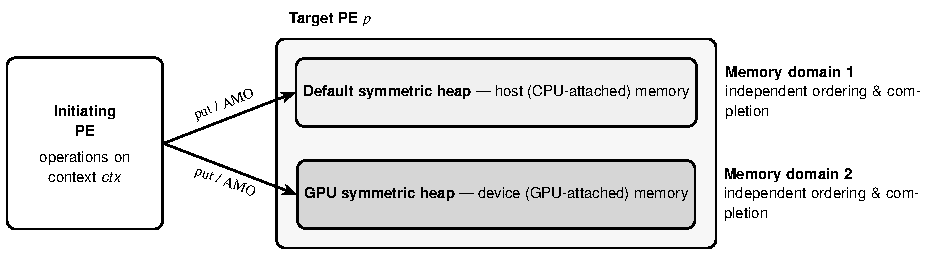
\includegraphics{figures/fig-mem-domains.pdf}
\caption{Each PE exposes two independent \emph{memory domains}: the default
symmetric heap in host (CPU-attached) memory and the GPU symmetric heap in device
(GPU-attached) memory. When GPU-aware communication is enabled, ordering and
completion are defined per memory domain: \FUNC{shmem\_fence} orders delivery
within one domain at a given PE, while \FUNC{shmem\_quiet} completes operations
and makes them visible across both domains at all PEs.}
\label{fig:mem-domains}
\end{figure}

\subsubsection{SHMEM\_FENCE}\label{subsec:ga_shmem_fence}

Ensures ordering of delivery of put, nonblocking get, \ac{AMO}, memory store, and put-with-signal
operations on symmetric data objects in the same memory domain when GPU-aware communication is enabled.

\begin{apidefinition}
\begin{Csynopsis}
void shmem_fence(void);
void shmem_ctx_fence(shmem_ctx_t ctx);
\end{Csynopsis}

\begin{apiarguments}
\apiargument{IN}{ctx}{A context handle specifying the context on which to perform
the operation. When this argument is not provided, the operation is performed on
the default context.}
\end{apiarguments}

\apidescription{
The \FUNC{shmem\_fence} routine ensures ordering of delivery of put, \ac{AMO},
memory store, and put-with-signal operations on symmetric data objects. All such
operations on symmetric data objects issued to a memory domain on a particular \ac{PE} on the given
context prior to the call to \FUNC{shmem\_fence} are guaranteed to be delivered
before any subsequent such operations to the same domain on the same \ac{PE} on the same context.
\FUNC{shmem\_fence} guarantees order of delivery, not completion. It does not
guarantee order of delivery of nonblocking get or values fetched by nonblocking
\ac{AMO} routines.

Memory store operations include direct stores to symmetric data objects performed
through local pointers returned by \FUNC{shmem\_ptr} or
\FUNC{shmem\_team\_ptr}. When the target symmetric data object resides in the
\ac{GPU} symmetric heap, a direct store through such a pointer constitutes a
memory store to the \ac{GPU} symmetric heap.

When GPU-aware communication is enabled, \FUNC{shmem\_fence} retains the
per-target-PE ordering semantics defined in \openshmem 1.6. However, when two
operations issued by the same \ac{PE} target different memory domains on the same
target \ac{PE}, \FUNC{shmem\_fence} does not provide cross-domain visibility
guarantees.

If \VAR{ctx} has the value \CONST{SHMEM\_CTX\_INVALID}, no operation is
performed.
}

\apireturnvalues{
None.
}

\apinotes{
\FUNC{shmem\_fence} only provides per-PE ordering guarantees and does not
guarantee completion of delivery. When GPU-aware communication is in use,
\FUNC{shmem\_fence} is sufficient to order operations that target the same memory
domain on the same \ac{PE}. It is not sufficient to guarantee visibility when two
operations target different memory domains on the same \ac{PE}.

The \FUNC{shmem\_quiet} routine should be called if completion of put, \ac{AMO},
memory store, or put-with-signal operations on symmetric data objects is desired
when operations target different memory domains or when multiple target \acp{PE}
are involved.
}
\end{apidefinition}

\subsubsection{SHMEM\_QUIET}\label{subsec:ga_shmem_quiet}

Waits for completion of all outstanding put, \ac{AMO}, memory store, and
put-with-signal operations on symmetric data objects issued by a \ac{PE} when
GPU-aware communication is enabled.

\begin{apidefinition}
\begin{Csynopsis}
void shmem_quiet(void);
void shmem_ctx_quiet(shmem_ctx_t ctx);
\end{Csynopsis}

\begin{apiarguments}
\apiargument{IN}{ctx}{A context handle specifying the context on which to perform
the operation. When this argument is not provided, the operation is performed on
the default context.}
\end{apiarguments}

\apidescription{
The \FUNC{shmem\_quiet} routine ensures completion of all outstanding put,
\ac{AMO}, memory store, and put-with-signal operations on symmetric data objects
issued by the calling \ac{PE} on the given context. All such operations are
guaranteed to be complete and visible to all \acp{PE} when \FUNC{shmem\_quiet}
returns.

When GPU-aware communication is enabled, \FUNC{shmem\_quiet} ensures completion
and visibility of all prior operations to both the default symmetric heap and the
\ac{GPU} symmetric heap at their respective targets. The receiving \ac{PE} shall
perform appropriate host-device synchronization after observing data that
indicates completion before accessing data from a prior operation that resides in
GPU-attached memory.

If \VAR{ctx} has the value \CONST{SHMEM\_CTX\_INVALID}, no operation is
performed.
}

\apireturnvalues{
None.
}

\apinotes{
There is a subtle difference between \FUNC{shmem\_fence} and
\FUNC{shmem\_quiet}, in that \FUNC{shmem\_quiet} guarantees completion of all
operations on symmetric data objects, making the updates visible to all other
\acp{PE} across all memory domains, including the \ac{GPU} symmetric heap and the
default symmetric heap. \FUNC{shmem\_fence} provides only per-PE ordering within
a single memory domain and does not guarantee cross-domain visibility.
}
\end{apidefinition}

\begin{figure}[!ht]
\centering
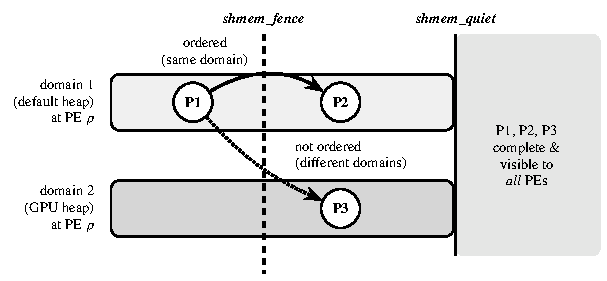
\includegraphics{figures/fig-fence-quiet.pdf}
\caption{Memory-domain-based ordering and completion. \FUNC{shmem\_fence}
guarantees that operations issued before it are delivered before operations
issued after it \emph{when they target the same memory domain at the same PE}
(P1 before P2). It provides no ordering between operations that target different
memory domains at the same PE (P1 and P3), and none across different PEs.
\FUNC{shmem\_quiet} completes all prior operations and makes them visible to all
PEs across both memory domains.}
\label{fig:fence-quiet}
\end{figure}

\subsubsection{SHMEM\_PUT\_SIGNAL}\label{subsec:ga_put_signal_ordering}

Copies data from a contiguous local data object to a data object on a specified
\ac{PE} and subsequently updates a remote flag to signal completion. The
put-with-signal routines guarantee ordering between the data delivery and the
signal update within a single operation, including when the data and the signal
target different memory domains.

\begin{apidefinition}
\begin{Csynopsis}
void shmem_put_signal(TYPE *dest, const TYPE *source, size_t nelems,
    uint64_t *sig_addr, uint64_t signal, int sig_op, int pe);
void shmem_ctx_put_signal(shmem_ctx_t ctx, TYPE *dest, const TYPE *source,
    size_t nelems, uint64_t *sig_addr, uint64_t signal, int sig_op, int pe);
\end{Csynopsis}

\begin{apiarguments}
\apiargument{IN}{ctx}{A context handle specifying the context on which to perform
the operation.}
\apiargument{OUT}{dest}{Symmetric address of the data object to be updated on the
remote PE.}
\apiargument{IN}{source}{Local address of the data object containing the data to
be copied.}
\apiargument{IN}{nelems}{Number of elements in the \VAR{dest} and \VAR{source}
arrays.}
\apiargument{OUT}{sig\_addr}{Symmetric address of the signal data object to be
updated on the remote PE as a signal.}
\apiargument{IN}{signal}{Unsigned 64-bit value used for updating the remote
\VAR{sig\_addr}.}
\apiargument{IN}{sig\_op}{Signal operator for the update on \VAR{sig\_addr}.}
\apiargument{IN}{pe}{PE number of the remote PE.}
\end{apiarguments}

\apidescription{
When GPU-aware communication is enabled, the \VAR{dest} data object and the
\VAR{sig\_addr} signal data object may reside in different memory domains on the
same target \ac{PE}. The \VAR{dest} data object may reside in the \ac{GPU}
symmetric heap and the \VAR{sig\_addr} signal data object may reside in the
default symmetric heap, or the reverse. The put-with-signal routine guarantees
that the data is delivered to the \VAR{dest} data object before the signal update
is visible at the \VAR{sig\_addr} signal data object, regardless of whether the
two objects reside in the same or different memory domains.

This cross-domain ordering guarantee is specific to the put-with-signal routine.
It does not extend to ordering between a put-with-signal routine and other
independent operations.
}

\apireturnvalues{
None.
}

\apinotes{
Unlike the case where two independent operations target different memory domains,
the put-with-signal routine provides cross-domain ordering between its data
delivery and signal update as a single atomic-like operation.
\FUNC{shmem\_fence} does not provide equivalent cross-domain ordering for two
independent operations.
}
\end{apidefinition}

\begin{figure}[!ht]
\centering
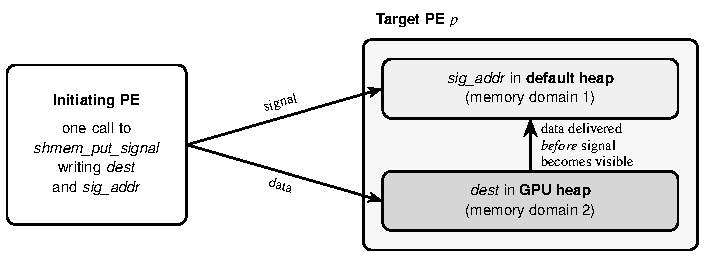
\includegraphics{figures/fig-put-signal-xdomain.pdf}
\caption{Cross-domain ordering of \FUNC{shmem\_put\_signal}. A single
put-with-signal operation guarantees that the data written to \textit{dest} is
delivered before the signal update at \textit{sig\_addr} becomes visible, even
when \textit{dest} and \textit{sig\_addr} reside in different memory domains at
the target PE. Two independent operations ordered with \FUNC{shmem\_fence} do
not provide this cross-domain guarantee.}
\label{fig:put-signal-xdomain}
\end{figure}

\subsubsection{Global Synchronization}\label{subsec:ga_barrier}

\begin{apidefinition}
\begin{Csynopsis}
void shmem_barrier_all(void);
void shmem_barrier(int PE_start, int logPE_stride, int PE_size, long *pSync);
\end{Csynopsis}

\begin{apiarguments}
\apiargument{IN}{PE\_start}{The lowest PE number of the active set of PEs.}
\apiargument{IN}{logPE\_stride}{The log (base 2) of the stride between
consecutive PE numbers in the active set.}
\apiargument{IN}{PE\_size}{The number of PEs in the active set.}
\apiargument{IN}{pSync}{Symmetric address of a work array of size at least
\CONST{SHMEM\_BARRIER\_SYNC\_SIZE}.}
\end{apiarguments}

\apidescription{
When GPU-aware communication is enabled, the implicit completion semantics of
\FUNC{shmem\_barrier\_all} and \FUNC{shmem\_barrier} are equivalent to calling
\FUNC{shmem\_quiet} on the default context prior to synchronization. All prior
operations to both the default symmetric heap and the \ac{GPU} symmetric heap are
guaranteed to be complete and visible to all \acp{PE} when the barrier returns,
regardless of whether the operations target different memory domains or different
\acp{PE}.
}

\apireturnvalues{
None.
}

\apinotes{
The \FUNC{shmem\_barrier\_all} routine is equivalent to calling
\FUNC{shmem\_ctx\_quiet} on the default context followed by calling
\FUNC{shmem\_team\_sync} on the world team.

The \FUNC{shmem\_team\_sync} routine, in contrast with the barrier routines, only
ensures completion and visibility of previously issued memory stores and does not
ensure completion of remote memory updates issued through \openshmem routines.
}
\end{apidefinition}



% Section 16: GPU-Centric Communication

\section{GPU-Centric Communication}\label{sec:gpu_centric}

This section defines routines that shall be invoked from within \ac{GPU} device
kernels. Calling these routines from the host results in \textbf{undefined
behavior}.

The \openshmem library shall have been initialized with
\CONST{SHMEM\_DEVICE\_KERNEL\_INIT} and the corresponding capability shall have
been returned in the \VAR{provided} argument of \FUNC{shmem\_init\_thread}.
Calling any routine in this section without the required initialization results
in \textbf{undefined behavior}.

All routines in this section use the \texttt{shmemg\_} prefix and operate on
symmetric data objects allocated from the \ac{GPU} symmetric heap. A symmetric
address and a target \ac{PE} identifier are used to address remote data objects.
Unless otherwise noted, any \ac{GPU} thread within a device kernel may call these
routines.

In the synopses that follow, the \CONST{SHMEMG\_DEVICE} annotation
(\cref{subsec:shmemg_device}) marks each routine as callable from a \ac{GPU}
device kernel. It expands to the execution-space qualifier required by the
compilation environment, or to no tokens where none is required. The code
examples in this specification use CUDA syntax, such as \texttt{\_\_global\_\_}
kernels and vendor-specific kernel-launch syntax, for concreteness; equivalent
constructs apply in other \ac{GPU} programming environments.


\subsection{Library Setup and Query}\label{subsec:gc_setup}

\subsubsection{SHMEMG\_MY\_PE}\label{subsec:shmemg_my_pe}

Returns the \ac{PE} number of the calling \ac{PE}.

\begin{apidefinition}
\begin{Csynopsis}
SHMEMG_DEVICE int shmemg_my_pe(void);
\end{Csynopsis}

\begin{apiarguments}
None.
\end{apiarguments}

\apidescription{
Callable from within a \ac{GPU} kernel.
The \FUNC{shmemg\_my\_pe} routine returns the \ac{PE} number of the calling
\ac{PE}. The value is an integer between 0 and \texttt{npes - 1}, where
\texttt{npes} is the total number of \acp{PE} in the program. The returned value
is identical to the value returned by \FUNC{shmem\_my\_pe} on the host for the
same \ac{PE}.
}

\apireturnvalues{
Integer --- between 0 and \texttt{npes - 1}.
}

\apinotes{
All threads within a kernel launched by the same \ac{PE} shall observe the same
return value.
}
\end{apidefinition}

\subsubsection{SHMEMG\_N\_PES}\label{subsec:shmemg_n_pes}

Returns the number of \acp{PE} in the \openshmem program.

\begin{apidefinition}
\begin{Csynopsis}
SHMEMG_DEVICE int shmemg_n_pes(void);
\end{Csynopsis}

\begin{apiarguments}
None.
\end{apiarguments}

\apidescription{
Callable from within a \ac{GPU} kernel.
The \FUNC{shmemg\_n\_pes} routine returns the total number of \acp{PE} in the
\openshmem program. The returned value is identical to the value returned by
\FUNC{shmem\_n\_pes} on the host.
}

\apireturnvalues{
Integer --- total number of \acp{PE} in the program.
}

\apinotes{
All threads within a kernel launched by the same \ac{PE} shall observe the same
return value.
}
\end{apidefinition}

\paragraph*{\textbf{Example}}\mbox{}\par\nobreak
The following program launches a device kernel that queries the calling \ac{PE}
number and the total number of \acp{PE} from within the kernel using
\FUNC{shmemg\_my\_pe} and \FUNC{shmemg\_n\_pes}, writing the results to a
symmetric buffer in the \ac{GPU} symmetric heap.

\lstinputlisting[style=SourceListingsDefault]{example_code/gc_setup_example.c}

\subsubsection{SHMEMG\_PTR}\label{subsec:shmemg_ptr}

Returns a pointer to a symmetric data object on a specified \ac{PE} that is
directly accessible from within a \ac{GPU} kernel.

\begin{apidefinition}
\begin{Csynopsis}
SHMEMG_DEVICE void *shmemg_ptr(const void *dest, int pe);
\end{Csynopsis}

\begin{apiarguments}
\apiargument{IN}{dest}{Symmetric address of the remotely accessible data object
to be referenced. Shall reside in the \ac{GPU} symmetric heap.}
\apiargument{IN}{pe}{PE number of the remote PE.}
\end{apiarguments}

\apidescription{
Callable from within a \ac{GPU} kernel.
The \FUNC{shmemg\_ptr} routine returns an address that may be used to directly
reference the symmetric data object \VAR{dest} on \ac{PE} \VAR{pe} from within a
\ac{GPU} kernel. This address can be used by the calling \ac{GPU} thread to
perform ordinary loads and stores to the remote data object, bypassing the
\ac{RMA} routines. This is the \ac{GPU}-centric analogue of \FUNC{shmem\_ptr}
in the \openshmem specification.

The routine returns a valid address only when the symmetric data object on the
remote \ac{PE} \VAR{pe} is directly accessible from the calling \ac{PE}'s
\ac{GPU}, for example when the remote \ac{PE} resides on the same node and its
symmetric heap is mapped into the accessing \ac{GPU}'s address space. When the
remote data object is not directly accessible, the routine returns a null
pointer.

Accesses performed through a pointer returned by \FUNC{shmemg\_ptr} are not
ordered or completed by \FUNC{shmemg\_fence} or \FUNC{shmemg\_quiet} with
respect to \ac{RMA} operations. Ordering and visibility of such direct accesses
are governed by the memory model of the underlying \ac{GPU} and the memory
ordering routines described in Section~\ref{subsec:gc_ordering}.
}

\apireturnvalues{
A pointer to the symmetric data object \VAR{dest} on \ac{PE} \VAR{pe} when that
object is directly accessible from the calling \ac{PE}'s \ac{GPU}; otherwise a
null pointer.
}

\apinotes{
\FUNC{shmemg\_ptr} operates at single-thread granularity. No thread group or
hardware thread group variants are defined. When \VAR{pe} is the calling \ac{PE},
\FUNC{shmemg\_ptr} returns a pointer to the local symmetric data object.
}
\end{apidefinition}

\paragraph*{\textbf{Example}}\mbox{}\par\nobreak
The following program uses \FUNC{shmemg\_ptr} to obtain a directly accessible
pointer to a symmetric buffer on the right neighbor \ac{PE}. When the neighbor
is directly accessible, the kernel writes into the remote buffer with an
ordinary store through the returned pointer; otherwise it falls back to
\FUNC{shmemg\_putmem}.

\lstinputlisting[style=SourceListingsDefault]{example_code/gc_ptr_example.c}


\subsection{Context Management}\label{subsec:gc_context}

Only communication contexts associated with \CONST{SHMEM\_DEVICE\_TEAM\_WORLD},
\CONST{SHMEM\_DEVICE\_TEAM\_SHARED}, or teams created from either of them through
\FUNC{shmem\_team\_split\_strided} and \FUNC{shmem\_team\_split\_2d} routines are
capable of performing GPU-centric communication operations from within \ac{GPU}
kernels. Using a context associated with any other team for GPU-centric
operations results in \textbf{undefined behavior}.

\CONST{SHMEM\_DEVICE\_CTX\_DEFAULT} is a predefined communication context of
type \CTYPE{shmem\_ctx\_t} associated with \CONST{SHMEM\_DEVICE\_TEAM\_WORLD}.
All GPU-centric communication operations and synchronizations that do not specify
a context shall be performed on \CONST{SHMEM\_DEVICE\_CTX\_DEFAULT}. \ac{GPU}
threads may pass \CONST{SHMEM\_DEVICE\_CTX\_DEFAULT} to any device-callable
routine that accepts a context argument.

Explicit device contexts are created on the host using \FUNC{shmem\_ctx\_create}
or \FUNC{shmem\_team\_create\_ctx} with the \CONST{SHMEM\_DEVICE\_CTX} option. A
context created with \FUNC{shmem\_ctx\_create} is associated with
\CONST{SHMEM\_DEVICE\_TEAM\_WORLD}. For \FUNC{shmem\_team\_create\_ctx}, the team
argument shall be an existing device team. Once created, these contexts may be
passed to device-callable routines from within \ac{GPU} kernels. Device contexts
shall not be created or destroyed from within \ac{GPU} kernels.

Using a device context for GPU-aware (host-initiated) operations, or using a
non-device context (including \CONST{SHMEM\_CTX\_DEFAULT}) for GPU-centric
operations, results in \textbf{undefined behavior}.

\paragraph*{\textbf{Example}}\mbox{}\par\nobreak
The following program creates an explicit device context on the host from
\CONST{SHMEM\_DEVICE\_TEAM\_WORLD} with the \CONST{SHMEM\_DEVICE\_CTX} option,
passes it to a device kernel that issues a context-qualified put and completes it
with \FUNC{shmemg\_ctx\_quiet}, and destroys the context on the host. Device
contexts are created and destroyed only on the host.

\lstinputlisting[style=SourceListingsDefault]{example_code/gc_context_example.c}


\subsection{Communication Operations}\label{subsec:gc_comm_ops}

The source and destination buffers for all data movement operations and the
symmetric data objects for all synchronization operations in this section shall
reside in the \ac{GPU} symmetric heap. Using local \ac{GPU} memory, local CPU
memory, or memory from the default symmetric heap as source, destination, or
synchronization operands for GPU-centric communication operations results in
\textbf{undefined behavior}.

For routines with a \VAR{pe} argument, the \VAR{pe} argument shall identify a
\ac{PE} in the team associated with the given \VAR{ctx} when provided, or the
default context otherwise. Passing an invalid \ac{PE} number results in
\textbf{undefined behavior}.

Each communication routine is provided at three thread granularities:

\begin{longtable}{|p{3cm}|p{3cm}|p{8.5cm}|}
\hline
\textbf{Suffix} & \textbf{Granularity} & \textbf{Description} \\
\hline
\endfirsthead
\hline
\textbf{Suffix} & \textbf{Granularity} & \textbf{Description} \\
\hline
\endhead
\emph{(none)} & Thread & A single \ac{GPU} thread initiates the operation. \\
\hline
\texttt{\_tg} & Thread group & All threads in a thread group collectively initiate
the operation (e.g., a thread block or workgroup). \\
\hline
\texttt{\_htg} & Hardware thread group & All threads in a hardware thread group
collectively initiate the operation (e.g., a warp or wavefront). \\
\hline
\end{longtable}

The thread group (\texttt{\_tg}) and hardware thread group (\texttt{\_htg})
variants are collective across the threads in the specified group. All
participating threads shall call the routine with the same arguments. If any
thread in the group does not participate, or if arguments differ across threads,
the behavior is undefined.

The atomic memory operations (\cref{subsec:gc_amo}) and point-to-point
synchronization routines (\cref{subsec:gc_p2p}) are provided as typed variants,
following the naming convention of the \openshmem 1.6 specification. In the name
of a typed routine, \TYPENAME{} is the type-name component that identifies the
operand type, while \TYPE{} is the corresponding C type used in the routine
signature. The supported types and the \TYPE{}-to-\TYPENAME{} correspondence are
those defined by the \openshmem 1.6 specification for the relevant operation
category. For example, the type \TYPE{} \KEYWORD{unsigned long long} has
\TYPENAME{} \texttt{ulonglong}, giving rise to routines such as
\FUNC{shmemg\_ulonglong\_atomic\_add}.


\subsubsection{Remote Memory Access (RMA)}\label{subsec:gc_rma}

The \ac{RMA} routines in this section transfer data between a local data object
and a symmetric data object on a remote \ac{PE}. The operations are one-sided:
the initiating \ac{GPU} thread provides all communication parameters and the
remote \ac{PE} need not participate.

The \VAR{source} and \VAR{dest} data objects shall reside in the \ac{GPU}
symmetric heap.

\subsubsubsection{\textbf{Blocking Put}}\label{subsec:gc_put}

Copies data from a contiguous local data object to a data object on a specified
\ac{PE}.

\begin{apidefinition}
\begin{Csynopsis}
SHMEMG_DEVICE void shmemg_putmem(void *dest, const void *source,
    size_t nelems, int pe);
SHMEMG_DEVICE void shmemg_ctx_putmem(shmem_ctx_t ctx, void *dest,
    const void *source, size_t nelems, int pe);
\end{Csynopsis}

Thread group variants:
\begin{CsynopsisCol}
SHMEMG_DEVICE void shmemg_putmem_tg(void *dest, const void *source,
    size_t nelems, int pe);
SHMEMG_DEVICE void shmemg_ctx_putmem_tg(shmem_ctx_t ctx, void *dest,
    const void *source, size_t nelems, int pe);
\end{CsynopsisCol}

Hardware thread group variants:
\begin{CsynopsisCol}
SHMEMG_DEVICE void shmemg_putmem_htg(void *dest, const void *source,
    size_t nelems, int pe);
SHMEMG_DEVICE void shmemg_ctx_putmem_htg(shmem_ctx_t ctx, void *dest,
    const void *source, size_t nelems, int pe);
\end{CsynopsisCol}

\begin{apiarguments}
\apiargument{IN}{ctx}{A context handle. When not provided, the operation is
performed on \CONST{SHMEM\_DEVICE\_CTX\_DEFAULT}.}
\apiargument{OUT}{dest}{Symmetric address of the destination data object.}
\apiargument{IN}{source}{Local address of the data object containing the data to
be copied. Shall reside in the \ac{GPU} symmetric heap.}
\apiargument{IN}{nelems}{Number of bytes to be copied.}
\apiargument{IN}{pe}{PE number of the remote PE relative to the team associated
with the given \VAR{ctx} when provided, or the default context otherwise.}
\end{apiarguments}

\apidescription{
Callable from within a \ac{GPU} kernel.
The routines return after the data has been copied out of the \VAR{source} array
on the local \ac{PE}. Delivery of data into the \VAR{dest} data object on the
destination \ac{PE} may occur in any order. Two successive put routines may
deliver data out of order unless a call to \FUNC{shmemg\_fence} is introduced
between the two calls.
}

\apireturnvalues{
None.
}
\end{apidefinition}

\subsubsubsection{\textbf{Nonblocking Put}}\label{subsec:gc_put_nbi}

Initiates a nonblocking copy of data from a contiguous local data object to a
data object on a specified \ac{PE}.

\begin{apidefinition}
\begin{Csynopsis}
SHMEMG_DEVICE void shmemg_putmem_nbi(void *dest, const void *source,
    size_t nelems, int pe);
SHMEMG_DEVICE void shmemg_ctx_putmem_nbi(shmem_ctx_t ctx, void *dest,
    const void *source, size_t nelems, int pe);
\end{Csynopsis}

Thread group variants:
\begin{CsynopsisCol}
SHMEMG_DEVICE void shmemg_putmem_nbi_tg(void *dest, const void *source,
    size_t nelems, int pe);
SHMEMG_DEVICE void shmemg_ctx_putmem_nbi_tg(shmem_ctx_t ctx, void *dest,
    const void *source, size_t nelems, int pe);
\end{CsynopsisCol}

Hardware thread group variants:
\begin{CsynopsisCol}
SHMEMG_DEVICE void shmemg_putmem_nbi_htg(void *dest, const void *source,
    size_t nelems, int pe);
SHMEMG_DEVICE void shmemg_ctx_putmem_nbi_htg(shmem_ctx_t ctx, void *dest,
    const void *source, size_t nelems, int pe);
\end{CsynopsisCol}

\begin{apiarguments}
\apiargument{IN}{ctx}{A context handle. When not provided, the operation is
performed on \CONST{SHMEM\_DEVICE\_CTX\_DEFAULT}.}
\apiargument{OUT}{dest}{Symmetric address of the destination data object.}
\apiargument{IN}{source}{Local address of the object containing the data to be
copied. Shall reside in the \ac{GPU} symmetric heap.}
\apiargument{IN}{nelems}{Number of bytes to be copied.}
\apiargument{IN}{pe}{PE number of the remote PE relative to the team associated
with the given \VAR{ctx} when provided, or the default context otherwise.}
\end{apiarguments}

\apidescription{
Callable from within a \ac{GPU} kernel.
The routines return after initiating the operation. The operation is considered
complete after a subsequent call to \FUNC{shmemg\_quiet}. At the completion of
\FUNC{shmemg\_quiet}, the data has been copied into the \VAR{dest} array on the
destination \ac{PE}.
}

\apireturnvalues{
None.
}
\end{apidefinition}

\subsubsubsection{\textbf{Single-Element Put}}\label{subsec:gc_p}

Copies a single data element to a data object on a specified \ac{PE}.

\begin{apidefinition}
\begin{Csynopsis}
SHMEMG_DEVICE void shmemg_TYPENAME_p(TYPE *dest, TYPE value, int pe);
SHMEMG_DEVICE void shmemg_ctx_TYPENAME_p(shmem_ctx_t ctx, TYPE *dest,
    TYPE value, int pe);
\end{Csynopsis}

where \TYPE{} is one of the standard RMA types defined in \openshmem 1.6.

\begin{apiarguments}
\apiargument{IN}{ctx}{A context handle. When not provided, the operation is
performed on \CONST{SHMEM\_DEVICE\_CTX\_DEFAULT}.}
\apiargument{OUT}{dest}{Symmetric address of the destination data object. Shall
reside in the \ac{GPU} symmetric heap.}
\apiargument{IN}{value}{The value to be transferred to \VAR{dest}.}
\apiargument{IN}{pe}{PE number of the remote PE.}
\end{apiarguments}

\apidescription{
Callable from within a \ac{GPU} kernel.
The \FUNC{shmemg\_p} routines write \VAR{value} to the symmetric data object at
address \VAR{dest} on \ac{PE} \VAR{pe}. The \VAR{value} argument is passed by
value; no memory-location restriction applies to it. The routines return after
\VAR{value} has been copied out on the local \ac{PE}. Delivery of \VAR{value}
into the \VAR{dest} data object on the destination \ac{PE} may be ordered using
\FUNC{shmemg\_fence} and completed using \FUNC{shmemg\_quiet}, as for other put
operations.

All \FUNC{shmemg\_p} routines operate at single-thread granularity. No thread
group or hardware thread group variants are defined.
}

\apireturnvalues{
None.
}
\end{apidefinition}

\subsubsubsection{\textbf{Blocking Get}}\label{subsec:gc_get}

Copies a contiguous symmetric data object from a specified \ac{PE}.

\begin{apidefinition}
\begin{Csynopsis}
SHMEMG_DEVICE void shmemg_getmem(void *dest, const void *source,
    size_t nelems, int pe);
SHMEMG_DEVICE void shmemg_ctx_getmem(shmem_ctx_t ctx, void *dest,
    const void *source, size_t nelems, int pe);
\end{Csynopsis}

Thread group variants:
\begin{CsynopsisCol}
SHMEMG_DEVICE void shmemg_getmem_tg(void *dest, const void *source,
    size_t nelems, int pe);
SHMEMG_DEVICE void shmemg_ctx_getmem_tg(shmem_ctx_t ctx, void *dest,
    const void *source, size_t nelems, int pe);
\end{CsynopsisCol}

Hardware thread group variants:
\begin{CsynopsisCol}
SHMEMG_DEVICE void shmemg_getmem_htg(void *dest, const void *source,
    size_t nelems, int pe);
SHMEMG_DEVICE void shmemg_ctx_getmem_htg(shmem_ctx_t ctx, void *dest,
    const void *source, size_t nelems, int pe);
\end{CsynopsisCol}

\begin{apiarguments}
\apiargument{IN}{ctx}{A context handle. When not provided, the operation is
performed on \CONST{SHMEM\_DEVICE\_CTX\_DEFAULT}.}
\apiargument{OUT}{dest}{Local address of the data object to be updated. Shall
reside in the \ac{GPU} symmetric heap.}
\apiargument{IN}{source}{Symmetric address of the source data object.}
\apiargument{IN}{nelems}{Number of bytes to be copied.}
\apiargument{IN}{pe}{PE number of the remote PE relative to the team associated
with the given \VAR{ctx} when provided, or the default context otherwise.}
\end{apiarguments}

\apidescription{
Callable from within a \ac{GPU} kernel.
The routines copy a contiguous symmetric data object from \ac{PE} \VAR{pe} to the
local \VAR{dest} data object. The routines return after the data has been
delivered to the \VAR{dest} array on the local \ac{PE}.
}

\apireturnvalues{
None.
}
\end{apidefinition}

\subsubsubsection{\textbf{Nonblocking Get}}\label{subsec:gc_get_nbi}

Initiates a nonblocking copy of a contiguous symmetric data object from a
specified \ac{PE}.

\begin{apidefinition}
\begin{Csynopsis}
SHMEMG_DEVICE void shmemg_getmem_nbi(void *dest, const void *source,
    size_t nelems, int pe);
SHMEMG_DEVICE void shmemg_ctx_getmem_nbi(shmem_ctx_t ctx, void *dest,
    const void *source, size_t nelems, int pe);
\end{Csynopsis}

Thread group variants:
\begin{CsynopsisCol}
SHMEMG_DEVICE void shmemg_getmem_nbi_tg(void *dest, const void *source,
    size_t nelems, int pe);
SHMEMG_DEVICE void shmemg_ctx_getmem_nbi_tg(shmem_ctx_t ctx, void *dest,
    const void *source, size_t nelems, int pe);
\end{CsynopsisCol}

Hardware thread group variants:
\begin{CsynopsisCol}
SHMEMG_DEVICE void shmemg_getmem_nbi_htg(void *dest, const void *source,
    size_t nelems, int pe);
SHMEMG_DEVICE void shmemg_ctx_getmem_nbi_htg(shmem_ctx_t ctx, void *dest,
    const void *source, size_t nelems, int pe);
\end{CsynopsisCol}

\begin{apiarguments}
\apiargument{IN}{ctx}{A context handle. When not provided, the operation is
performed on \CONST{SHMEM\_DEVICE\_CTX\_DEFAULT}.}
\apiargument{OUT}{dest}{Local address of the data object to be updated. Shall
reside in the \ac{GPU} symmetric heap.}
\apiargument{IN}{source}{Symmetric address of the source data object.}
\apiargument{IN}{nelems}{Number of bytes to be copied.}
\apiargument{IN}{pe}{PE number of the remote PE relative to the team associated
with the given \VAR{ctx} when provided, or the default context otherwise.}
\end{apiarguments}

\apidescription{
Callable from within a \ac{GPU} kernel.
The routines initiate a copy of a contiguous symmetric data object from \ac{PE}
\VAR{pe} to the local \VAR{dest} data object. The routines return after
initiating the operation. The operation is considered complete after a subsequent
call to \FUNC{shmemg\_quiet}. At the completion of \FUNC{shmemg\_quiet}, the
data has been delivered to the \VAR{dest} array on the local \ac{PE}.
}

\apireturnvalues{
None.
}
\end{apidefinition}

\subsubsubsection{\textbf{Single-Element Get}}\label{subsec:gc_g}

Copies a single data element from a data object on a specified \ac{PE}.

\begin{apidefinition}
\begin{Csynopsis}
SHMEMG_DEVICE TYPE shmemg_TYPENAME_g(const TYPE *source, int pe);
SHMEMG_DEVICE TYPE shmemg_ctx_TYPENAME_g(shmem_ctx_t ctx,
    const TYPE *source, int pe);
\end{Csynopsis}

where \TYPE{} is one of the standard RMA types defined in \openshmem 1.6.

\begin{apiarguments}
\apiargument{IN}{ctx}{A context handle. When not provided, the operation is
performed on \CONST{SHMEM\_DEVICE\_CTX\_DEFAULT}.}
\apiargument{IN}{source}{Symmetric address of the source data object. Shall reside
in the \ac{GPU} symmetric heap.}
\apiargument{IN}{pe}{PE number of the remote PE.}
\end{apiarguments}

\apidescription{
Callable from within a \ac{GPU} kernel.
The \FUNC{shmemg\_g} routines read the value of the symmetric data object at
address \VAR{source} on \ac{PE} \VAR{pe} and return it to the calling \ac{GPU}
thread. The routines return after the value has been delivered to the calling
thread. The returned value is passed by value; no memory-location restriction
applies to it.

All \FUNC{shmemg\_g} routines operate at single-thread granularity. No thread
group or hardware thread group variants are defined.
}

\apireturnvalues{
The value of the symmetric data object at address \VAR{source} on \ac{PE}
\VAR{pe}, of type \TYPE{}.
}
\end{apidefinition}

\paragraph*{\textbf{Example}}\mbox{}\par\nobreak
In the following program each \ac{PE} launches a device kernel that puts one
element into its right neighbor's symmetric buffer with \FUNC{shmemg\_putmem}
and completes the transfer with \FUNC{shmemg\_quiet}. Both the source and
destination operands reside in the \ac{GPU} symmetric heap.

\lstinputlisting[style=SourceListingsDefault]{example_code/gc_rma_example.c}
\paragraph*{\textbf{Example}}\mbox{}\par\nobreak
The following program uses \FUNC{shmemg\_ptr} to obtain a directly accessible
pointer to a symmetric buffer on the right neighbor \ac{PE}. When the neighbor
is directly accessible, the kernel writes into the remote buffer with an
ordinary store through the returned pointer; otherwise it falls back to
\FUNC{shmemg\_putmem}.

\lstinputlisting[style=SourceListingsDefault]{example_code/gc_ptr_example.c}

\subsubsection{Atomic Memory Operations (AMO)}\label{subsec:gc_amo}

The \ac{AMO} routines in this section perform atomic read, update, or write
operations on symmetric data objects in the \ac{GPU} symmetric heap. Two types
are defined: non-fetching routines update the remote data object without
returning a value, and fetching routines return the value of the remote data
object prior to the update.

The \VAR{dest} data object for all \ac{AMO} routines in this section shall reside
in the \ac{GPU} symmetric heap. Using local \ac{GPU} memory, local CPU memory, or
memory from the default symmetric heap as the \VAR{dest} operand results in
\textbf{undefined behavior}.

The \VAR{value}, \VAR{cond}, and \VAR{cmp\_value} arguments are passed by value;
no memory location restriction applies.

All \ac{AMO} routines operate at single-thread granularity. No thread group or
hardware thread group variants are defined.

\subsubsubsection{\textbf{Non-fetching AMOs}}\label{subsec:gc_nonfetch_amo}

Atomically updates a symmetric data object on a specified \ac{PE}.

\begin{apidefinition}
\begin{Csynopsis}
SHMEMG_DEVICE void shmemg_TYPENAME_atomic_set(TYPE *dest, TYPE value, int pe);
SHMEMG_DEVICE void shmemg_ctx_TYPENAME_atomic_set(shmem_ctx_t ctx,
    TYPE *dest, TYPE value, int pe);

SHMEMG_DEVICE void shmemg_TYPENAME_atomic_add(TYPE *dest, TYPE value, int pe);
SHMEMG_DEVICE void shmemg_ctx_TYPENAME_atomic_add(shmem_ctx_t ctx,
    TYPE *dest, TYPE value, int pe);

SHMEMG_DEVICE void shmemg_TYPENAME_atomic_inc(TYPE *dest, int pe);
SHMEMG_DEVICE void shmemg_ctx_TYPENAME_atomic_inc(shmem_ctx_t ctx,
    TYPE *dest, int pe);

SHMEMG_DEVICE void shmemg_TYPENAME_atomic_and(TYPE *dest, TYPE value, int pe);
SHMEMG_DEVICE void shmemg_ctx_TYPENAME_atomic_and(shmem_ctx_t ctx,
    TYPE *dest, TYPE value, int pe);

SHMEMG_DEVICE void shmemg_TYPENAME_atomic_or(TYPE *dest, TYPE value, int pe);
SHMEMG_DEVICE void shmemg_ctx_TYPENAME_atomic_or(shmem_ctx_t ctx,
    TYPE *dest, TYPE value, int pe);

SHMEMG_DEVICE void shmemg_TYPENAME_atomic_xor(TYPE *dest, TYPE value, int pe);
SHMEMG_DEVICE void shmemg_ctx_TYPENAME_atomic_xor(shmem_ctx_t ctx,
    TYPE *dest, TYPE value, int pe);
\end{Csynopsis}

where \TYPE{} is one of the standard AMO types defined in \openshmem 1.6, and
\TYPENAME{} is the corresponding type-name component of the routine name.

\begin{apiarguments}
\apiargument{IN}{ctx}{A context handle. When not provided, the operation is
performed on \CONST{SHMEM\_DEVICE\_CTX\_DEFAULT}.}
\apiargument{OUT}{dest}{Symmetric address of the data object to be updated on the
remote PE. Shall reside in the \ac{GPU} symmetric heap.}
\apiargument{IN}{value}{The operand to the atomic operation. Not used by
\FUNC{shmemg\_atomic\_inc}.}
\apiargument{IN}{pe}{PE number of the remote PE relative to the team associated
with the given \VAR{ctx} when provided, or the default context otherwise.}
\end{apiarguments}

\apidescription{
Callable from within a \ac{GPU} kernel.
The non-fetching \ac{AMO} routines perform an atomic update to the data object at
address \VAR{dest} on \ac{PE} \VAR{pe}. The operations are:

\begin{longtable}{|p{5cm}|p{9.5cm}|}
\hline
\textbf{Routine} & \textbf{Operation} \\
\hline
\FUNC{shmemg\_atomic\_set} & Atomically sets the value at \VAR{dest} to \VAR{value}. \\
\hline
\FUNC{shmemg\_atomic\_add} & Atomically adds \VAR{value} to the value at \VAR{dest}. \\
\hline
\FUNC{shmemg\_atomic\_inc} & Atomically increments the value at \VAR{dest} by one. \\
\hline
\FUNC{shmemg\_atomic\_and} & Atomically performs a bitwise AND of \VAR{value} with the value at \VAR{dest}. \\
\hline
\FUNC{shmemg\_atomic\_or} & Atomically performs a bitwise OR of \VAR{value} with the value at \VAR{dest}. \\
\hline
\FUNC{shmemg\_atomic\_xor} & Atomically performs a bitwise XOR of \VAR{value} with the value at \VAR{dest}. \\
\hline
\end{longtable}

The routines return after the atomic update has been issued. Two successive
non-fetching \ac{AMO} routines may update the remote data object out of order
unless a call to \FUNC{shmemg\_fence} is introduced between the two calls.
}

\apireturnvalues{
None.
}
\end{apidefinition}

\subsubsubsection{\textbf{Fetching AMOs}}\label{subsec:gc_fetch_amo}

Atomically fetches or updates a symmetric data object on a specified \ac{PE} and
returns the prior value.

\begin{apidefinition}
\begin{Csynopsis}
SHMEMG_DEVICE TYPE shmemg_TYPENAME_atomic_fetch(const TYPE *source, int pe);
SHMEMG_DEVICE TYPE shmemg_ctx_TYPENAME_atomic_fetch(shmem_ctx_t ctx,
    const TYPE *source, int pe);

SHMEMG_DEVICE TYPE shmemg_TYPENAME_atomic_swap(TYPE *dest, TYPE value, int pe);
SHMEMG_DEVICE TYPE shmemg_ctx_TYPENAME_atomic_swap(shmem_ctx_t ctx,
    TYPE *dest, TYPE value, int pe);

SHMEMG_DEVICE TYPE shmemg_TYPENAME_atomic_compare_swap(TYPE *dest,
    TYPE cond, TYPE value, int pe);
SHMEMG_DEVICE TYPE shmemg_ctx_TYPENAME_atomic_compare_swap(shmem_ctx_t ctx,
    TYPE *dest, TYPE cond, TYPE value, int pe);

SHMEMG_DEVICE TYPE shmemg_TYPENAME_atomic_fetch_add(TYPE *dest,
    TYPE value, int pe);
SHMEMG_DEVICE TYPE shmemg_ctx_TYPENAME_atomic_fetch_add(shmem_ctx_t ctx,
    TYPE *dest, TYPE value, int pe);

SHMEMG_DEVICE TYPE shmemg_TYPENAME_atomic_fetch_inc(TYPE *dest, int pe);
SHMEMG_DEVICE TYPE shmemg_ctx_TYPENAME_atomic_fetch_inc(shmem_ctx_t ctx,
    TYPE *dest, int pe);

SHMEMG_DEVICE TYPE shmemg_TYPENAME_atomic_fetch_and(TYPE *dest,
    TYPE value, int pe);
SHMEMG_DEVICE TYPE shmemg_ctx_TYPENAME_atomic_fetch_and(shmem_ctx_t ctx,
    TYPE *dest, TYPE value, int pe);

SHMEMG_DEVICE TYPE shmemg_TYPENAME_atomic_fetch_or(TYPE *dest,
    TYPE value, int pe);
SHMEMG_DEVICE TYPE shmemg_ctx_TYPENAME_atomic_fetch_or(shmem_ctx_t ctx,
    TYPE *dest, TYPE value, int pe);

SHMEMG_DEVICE TYPE shmemg_TYPENAME_atomic_fetch_xor(TYPE *dest,
    TYPE value, int pe);
SHMEMG_DEVICE TYPE shmemg_ctx_TYPENAME_atomic_fetch_xor(shmem_ctx_t ctx,
    TYPE *dest, TYPE value, int pe);
\end{Csynopsis}

where \TYPE{} is one of the standard AMO types defined in \openshmem 1.6, and
\TYPENAME{} is the corresponding type-name component of the routine name.

\begin{apiarguments}
\apiargument{IN}{ctx}{A context handle. When not provided, the operation is
performed on \CONST{SHMEM\_DEVICE\_CTX\_DEFAULT}.}
\apiargument{OUT}{dest or source}{Symmetric address of the data object on the
remote PE. Shall reside in the \ac{GPU} symmetric heap.}
\apiargument{IN}{value}{The operand to the atomic operation. Not used by
\FUNC{shmemg\_atomic\_fetch} and \FUNC{shmemg\_atomic\_fetch\_inc}.}
\apiargument{IN}{cond}{The operand to be compared with the remote value. Used
only by \FUNC{shmemg\_atomic\_compare\_swap}.}
\apiargument{IN}{pe}{PE number of the remote PE relative to the team associated
with the given \VAR{ctx} when provided, or the default context otherwise.}
\end{apiarguments}

\apidescription{
Callable from within a \ac{GPU} kernel.
The fetching \ac{AMO} routines perform an atomic read or update to the data
object at address \VAR{dest} on \ac{PE} \VAR{pe} and return the prior value. The
operations are:

\begin{longtable}{|p{5.5cm}|p{9cm}|}
\hline
\textbf{Routine} & \textbf{Operation} \\
\hline
\FUNC{shmemg\_atomic\_fetch} & Atomically fetches the value at \VAR{source}. \\
\hline
\FUNC{shmemg\_atomic\_swap} & Atomically swaps the value at \VAR{dest} with \VAR{value} and returns the prior value. \\
\hline
\FUNC{shmemg\_atomic\_compare\_swap} & Compares the value at \VAR{dest} with \VAR{cond}; if equal, replaces it with \VAR{value}. Returns the prior value. \\
\hline
\FUNC{shmemg\_atomic\_fetch\_add} & Atomically adds \VAR{value} to \VAR{dest} and returns the prior value. \\
\hline
\FUNC{shmemg\_atomic\_fetch\_inc} & Atomically increments \VAR{dest} by one and returns the prior value. \\
\hline
\FUNC{shmemg\_atomic\_fetch\_and} & Atomically ANDs \VAR{value} with \VAR{dest} and returns the prior value. \\
\hline
\FUNC{shmemg\_atomic\_fetch\_or} & Atomically ORs \VAR{value} with \VAR{dest} and returns the prior value. \\
\hline
\FUNC{shmemg\_atomic\_fetch\_xor} & Atomically XORs \VAR{value} with \VAR{dest} and returns the prior value. \\
\hline
\end{longtable}

The routines return after the fetched value has been delivered to the calling
\ac{GPU} thread.
}

\apireturnvalues{
The value of the remote data object prior to the atomic operation, of type
\TYPE{}.
}
\end{apidefinition}

\subsubsubsection{\textbf{Nonblocking Fetching AMOs}}\label{subsec:gc_nbi_amo}

Initiates a nonblocking atomic fetch or update on a symmetric data object on a
specified \ac{PE}.

\begin{apidefinition}
\begin{Csynopsis}
SHMEMG_DEVICE void shmemg_TYPENAME_atomic_fetch_nbi(TYPE *fetch,
    const TYPE *source, int pe);
SHMEMG_DEVICE void shmemg_ctx_TYPENAME_atomic_fetch_nbi(shmem_ctx_t ctx,
    TYPE *fetch, const TYPE *source, int pe);

SHMEMG_DEVICE void shmemg_TYPENAME_atomic_swap_nbi(TYPE *fetch,
    TYPE *dest, TYPE value, int pe);
SHMEMG_DEVICE void shmemg_ctx_TYPENAME_atomic_swap_nbi(shmem_ctx_t ctx,
    TYPE *fetch, TYPE *dest, TYPE value, int pe);

SHMEMG_DEVICE void shmemg_TYPENAME_atomic_compare_swap_nbi(TYPE *fetch,
    TYPE *dest, TYPE cond, TYPE value, int pe);
SHMEMG_DEVICE void shmemg_ctx_TYPENAME_atomic_compare_swap_nbi(
    shmem_ctx_t ctx, TYPE *fetch, TYPE *dest, TYPE cond,
    TYPE value, int pe);

SHMEMG_DEVICE void shmemg_TYPENAME_atomic_fetch_add_nbi(TYPE *fetch,
    TYPE *dest, TYPE value, int pe);
SHMEMG_DEVICE void shmemg_ctx_TYPENAME_atomic_fetch_add_nbi(shmem_ctx_t ctx,
    TYPE *fetch, TYPE *dest, TYPE value, int pe);

SHMEMG_DEVICE void shmemg_TYPENAME_atomic_fetch_inc_nbi(TYPE *fetch,
    TYPE *dest, int pe);
SHMEMG_DEVICE void shmemg_ctx_TYPENAME_atomic_fetch_inc_nbi(shmem_ctx_t ctx,
    TYPE *fetch, TYPE *dest, int pe);

SHMEMG_DEVICE void shmemg_TYPENAME_atomic_fetch_and_nbi(TYPE *fetch,
    TYPE *dest, TYPE value, int pe);
SHMEMG_DEVICE void shmemg_ctx_TYPENAME_atomic_fetch_and_nbi(shmem_ctx_t ctx,
    TYPE *fetch, TYPE *dest, TYPE value, int pe);

SHMEMG_DEVICE void shmemg_TYPENAME_atomic_fetch_or_nbi(TYPE *fetch,
    TYPE *dest, TYPE value, int pe);
SHMEMG_DEVICE void shmemg_ctx_TYPENAME_atomic_fetch_or_nbi(shmem_ctx_t ctx,
    TYPE *fetch, TYPE *dest, TYPE value, int pe);

SHMEMG_DEVICE void shmemg_TYPENAME_atomic_fetch_xor_nbi(TYPE *fetch,
    TYPE *dest, TYPE value, int pe);
SHMEMG_DEVICE void shmemg_ctx_TYPENAME_atomic_fetch_xor_nbi(shmem_ctx_t ctx,
    TYPE *fetch, TYPE *dest, TYPE value, int pe);
\end{Csynopsis}

where \TYPE{} is one of the standard AMO types defined in \openshmem 1.6, and
\TYPENAME{} is the corresponding type-name component of the routine name.

\begin{apiarguments}
\apiargument{IN}{ctx}{A context handle. When not provided, the operation is
performed on \CONST{SHMEM\_DEVICE\_CTX\_DEFAULT}.}
\apiargument{OUT}{fetch}{Local address of the data object to be updated with the
fetched value. Shall reside in the \ac{GPU} symmetric heap.}
\apiargument{OUT}{dest or source}{Symmetric address of the data object on the
remote PE. Shall reside in the \ac{GPU} symmetric heap.}
\apiargument{IN}{value}{The operand to the atomic operation.}
\apiargument{IN}{cond}{The operand to be compared with the remote value. Used
only by \FUNC{shmemg\_atomic\_compare\_swap\_nbi}.}
\apiargument{IN}{pe}{PE number of the remote PE relative to the team associated
with the given \VAR{ctx} when provided, or the default context otherwise.}
\end{apiarguments}

\apidescription{
Callable from within a \ac{GPU} kernel.
The nonblocking fetching \ac{AMO} routines initiate an atomic fetch or update to
the data object at address \VAR{dest} on \ac{PE} \VAR{pe}. The routines return
after initiating the operation. The \VAR{fetch} data object shall not be accessed
until the operation has been completed by a subsequent call to
\FUNC{shmemg\_quiet}. Upon completion of \FUNC{shmemg\_quiet}, the prior value
of the remote data object has been written to \VAR{fetch} and the atomic update,
if any, has been performed.

The \VAR{fetch}, \VAR{dest}, and \VAR{source} data objects shall reside in the
\ac{GPU} symmetric heap.
}

\apireturnvalues{
None.
}
\end{apidefinition}

\paragraph*{\textbf{Example}}\mbox{}\par\nobreak
The following program has every \ac{PE} atomically fetch-and-add one to a shared
counter that lives on \ac{PE}~0 using \FUNC{shmemg\_long\_atomic\_fetch\_add},
obtaining a unique ticket value. The counter and the fetched result reside in the
\ac{GPU} symmetric heap.

\lstinputlisting[style=SourceListingsDefault]{example_code/gc_amo_example.c}


\subsubsection{Signaling Operations}\label{subsec:gc_signaling}

The signaling routines in this section copy data from a contiguous local data
object to a data object on a specified \ac{PE} and subsequently update a remote
signal data object to indicate delivery. The signal-fetch routine reads a local
signal value.

The \VAR{dest}, \VAR{sig\_addr}, and \VAR{source} data objects for all signaling
routines in this section shall reside in the \ac{GPU} symmetric heap. Using local
\ac{GPU} memory, local CPU memory, or memory from the default symmetric heap as
operands results in \textbf{undefined behavior}.

\subsubsubsection{\textbf{Put-with-Signal}}\label{subsec:gc_put_signal}

Copies data from a contiguous local data object to a data object on a specified
\ac{PE} and subsequently updates a remote signal data object.

\begin{apidefinition}
\begin{Csynopsis}
SHMEMG_DEVICE void shmemg_putmem_signal(void *dest, const void *source,
    size_t nelems, uint64_t *sig_addr, uint64_t signal,
    int sig_op, int pe);
SHMEMG_DEVICE void shmemg_ctx_putmem_signal(shmem_ctx_t ctx, void *dest,
    const void *source, size_t nelems, uint64_t *sig_addr,
    uint64_t signal, int sig_op, int pe);
\end{Csynopsis}

Thread group variants:
\begin{CsynopsisCol}
SHMEMG_DEVICE void shmemg_putmem_signal_tg(void *dest, const void *source,
    size_t nelems, uint64_t *sig_addr, uint64_t signal,
    int sig_op, int pe);
SHMEMG_DEVICE void shmemg_ctx_putmem_signal_tg(shmem_ctx_t ctx, void *dest,
    const void *source, size_t nelems, uint64_t *sig_addr,
    uint64_t signal, int sig_op, int pe);
\end{CsynopsisCol}

Hardware thread group variants:
\begin{CsynopsisCol}
SHMEMG_DEVICE void shmemg_putmem_signal_htg(void *dest, const void *source,
    size_t nelems, uint64_t *sig_addr, uint64_t signal,
    int sig_op, int pe);
SHMEMG_DEVICE void shmemg_ctx_putmem_signal_htg(shmem_ctx_t ctx, void *dest,
    const void *source, size_t nelems, uint64_t *sig_addr,
    uint64_t signal, int sig_op, int pe);
\end{CsynopsisCol}

\begin{apiarguments}
\apiargument{IN}{ctx}{A context handle. When not provided, the operation is
performed on \CONST{SHMEM\_DEVICE\_CTX\_DEFAULT}.}
\apiargument{OUT}{dest}{Symmetric address of the destination data object on the
remote PE.}
\apiargument{IN}{source}{Local address of the data object containing the data to
be copied. Shall reside in the \ac{GPU} symmetric heap.}
\apiargument{IN}{nelems}{Number of bytes to be copied.}
\apiargument{OUT}{sig\_addr}{Symmetric address of the signal data object on the
remote PE.}
\apiargument{IN}{signal}{Unsigned 64-bit value for updating \VAR{sig\_addr}.}
\apiargument{IN}{sig\_op}{Signal operator for the update on \VAR{sig\_addr}.}
\apiargument{IN}{pe}{PE number of the remote PE relative to the team associated
with the given \VAR{ctx} when provided, or the default context otherwise.}
\end{apiarguments}

\apidescription{
Callable from within a \ac{GPU} kernel.
The routines copy data from \VAR{source} to \VAR{dest} on \ac{PE} \VAR{pe} and
subsequently update the signal data object at \VAR{sig\_addr}. The routines
return after the data has been copied out of \VAR{source}. Completion of the
signal update on the remote \ac{PE} indicates delivery of the corresponding
\VAR{dest} data.

An update to the \VAR{sig\_addr} signal data object completes as if performed
atomically. The \VAR{dest}, \VAR{source}, and \VAR{sig\_addr} data objects shall
reside in the \ac{GPU} symmetric heap. \VAR{sig\_addr} and \VAR{dest} shall not
overlap in memory.
}

\apireturnvalues{
None.
}

\apinotes{
Completion of the signal update indicates only the delivery of the corresponding
\VAR{dest} data. Without a memory-ordering operation, there is no implied
ordering between the signal update and another data transfer.
}
\end{apidefinition}

\subsubsubsection{\textbf{Nonblocking Put-with-Signal}}\label{subsec:gc_put_signal_nbi}

Initiates a nonblocking copy of data to a specified \ac{PE} with a subsequent
signal update.

\begin{apidefinition}
\begin{Csynopsis}
SHMEMG_DEVICE void shmemg_putmem_signal_nbi(void *dest, const void *source,
    size_t nelems, uint64_t *sig_addr, uint64_t signal,
    int sig_op, int pe);
SHMEMG_DEVICE void shmemg_ctx_putmem_signal_nbi(shmem_ctx_t ctx, void *dest,
    const void *source, size_t nelems, uint64_t *sig_addr,
    uint64_t signal, int sig_op, int pe);
\end{Csynopsis}

Thread group variants:
\begin{CsynopsisCol}
SHMEMG_DEVICE void shmemg_putmem_signal_nbi_tg(void *dest, const void *source,
    size_t nelems, uint64_t *sig_addr, uint64_t signal,
    int sig_op, int pe);
SHMEMG_DEVICE void shmemg_ctx_putmem_signal_nbi_tg(shmem_ctx_t ctx,
    void *dest, const void *source, size_t nelems,
    uint64_t *sig_addr, uint64_t signal, int sig_op, int pe);
\end{CsynopsisCol}

Hardware thread group variants:
\begin{CsynopsisCol}
SHMEMG_DEVICE void shmemg_putmem_signal_nbi_htg(void *dest, const void *source,
    size_t nelems, uint64_t *sig_addr, uint64_t signal,
    int sig_op, int pe);
SHMEMG_DEVICE void shmemg_ctx_putmem_signal_nbi_htg(shmem_ctx_t ctx,
    void *dest, const void *source, size_t nelems,
    uint64_t *sig_addr, uint64_t signal, int sig_op, int pe);
\end{CsynopsisCol}

\begin{apiarguments}
\apiargument{IN}{ctx}{A context handle. When not provided, the operation is
performed on \CONST{SHMEM\_DEVICE\_CTX\_DEFAULT}.}
\apiargument{OUT}{dest}{Symmetric address of the destination data object.}
\apiargument{IN}{source}{Local address of the data object. Shall reside in the
\ac{GPU} symmetric heap.}
\apiargument{IN}{nelems}{Number of bytes to be copied.}
\apiargument{OUT}{sig\_addr}{Symmetric address of the signal data object.}
\apiargument{IN}{signal}{Unsigned 64-bit value for updating \VAR{sig\_addr}.}
\apiargument{IN}{sig\_op}{Signal operator for the update.}
\apiargument{IN}{pe}{PE number of the remote PE relative to the team associated
with the given \VAR{ctx} when provided, or the default context otherwise.}
\end{apiarguments}

\apidescription{
Callable from within a \ac{GPU} kernel.
The routines initiate a copy and a signal update. The routines return after
initiating the operation. The operation is considered complete after a subsequent
call to \FUNC{shmemg\_quiet}. The \VAR{dest}, \VAR{source}, and \VAR{sig\_addr}
data objects shall reside in the \ac{GPU} symmetric heap. \VAR{sig\_addr} and
\VAR{dest} shall not overlap in memory.
}

\apireturnvalues{
None.
}
\end{apidefinition}

\subsubsubsection{\textbf{Signal-Fetch}}\label{subsec:gc_signal_fetch}

Fetches the value of a local signal data object.

\begin{apidefinition}
\begin{Csynopsis}
SHMEMG_DEVICE uint64_t shmemg_signal_fetch(const uint64_t *sig_addr);
\end{Csynopsis}

\begin{apiarguments}
\apiargument{IN}{sig\_addr}{Local address of the remotely accessible signal
variable. Shall reside in the \ac{GPU} symmetric heap.}
\end{apiarguments}

\apidescription{
Callable from within a \ac{GPU} kernel.
\FUNC{shmemg\_signal\_fetch} returns the value of the signal data object at
address \VAR{sig\_addr} on the calling \ac{PE}. Access to \VAR{sig\_addr}
satisfies the atomicity guarantees described in the signaling operations
introduction.
}

\apireturnvalues{
The value of the signal data object at \VAR{sig\_addr} on the calling \ac{PE}.
}
\end{apidefinition}

\paragraph*{\textbf{Example}}\mbox{}\par\nobreak
The following program delivers a message from \ac{PE}~0 to \ac{PE}~1 with
\FUNC{shmemg\_putmem\_signal}, which writes the payload and then atomically
updates a remote signal object. \ac{PE}~1 polls its local signal with
\FUNC{shmemg\_signal\_fetch} until the arrival is observed. All operands reside
in the \ac{GPU} symmetric heap.

\lstinputlisting[style=SourceListingsDefault]{example_code/gc_signaling_example.c}


\subsubsection{Point-to-Point Synchronization}\label{subsec:gc_p2p}

The point-to-point synchronization routines block or test until a symmetric data
object on the local \ac{PE} satisfies a specified condition.

Each of these routines is also provided in thread group (\texttt{\_tg}) and
hardware thread group (\texttt{\_htg}) variants, as defined in
\cref{subsec:gc_comm_ops}. In these collective variants, all participating
threads return together once the condition is satisfied, and any return value is
the same across the group.

The \VAR{ivar} or \VAR{sig\_addr} data object shall reside in the \ac{GPU}
symmetric heap. Using local \ac{GPU} memory, local CPU memory, or memory from the
default symmetric heap results in \textbf{undefined behavior}.

\subsubsubsection{\textbf{Wait-Until}}\label{subsec:gc_wait_until}

Blocks until a symmetric data object on the local \ac{PE} satisfies a condition.

\begin{apidefinition}
\begin{Csynopsis}
SHMEMG_DEVICE void shmemg_TYPENAME_wait_until(TYPE *ivar, int cmp,
    TYPE cmp_value);
\end{Csynopsis}

Thread group variant:
\begin{CsynopsisCol}
SHMEMG_DEVICE void shmemg_TYPENAME_wait_until_tg(TYPE *ivar, int cmp,
    TYPE cmp_value);
\end{CsynopsisCol}

Hardware thread group variant:
\begin{CsynopsisCol}
SHMEMG_DEVICE void shmemg_TYPENAME_wait_until_htg(TYPE *ivar, int cmp,
    TYPE cmp_value);
\end{CsynopsisCol}

where \TYPE{} is one of the point-to-point synchronization types defined in
\openshmem 1.6, and \TYPENAME{} is the corresponding type-name component of the
routine name.

\begin{apiarguments}
\apiargument{IN}{ivar}{Symmetric address of the source data object. Shall reside
in the \ac{GPU} symmetric heap.}
\apiargument{IN}{cmp}{The comparison operator.}
\apiargument{IN}{cmp\_value}{The value against which \VAR{ivar} will be compared.}
\end{apiarguments}

\apidescription{
Callable from within a \ac{GPU} kernel.
\FUNC{shmemg\_wait\_until} blocks until the value of \VAR{ivar} at the calling
\ac{PE} satisfies the condition implied by \VAR{cmp} and \VAR{cmp\_value}. The
supported values of \VAR{cmp} are: \CONST{SHMEM\_CMP\_EQ},
\CONST{SHMEM\_CMP\_NE}, \CONST{SHMEM\_CMP\_GT}, \CONST{SHMEM\_CMP\_GE},
\CONST{SHMEM\_CMP\_LT}, and \CONST{SHMEM\_CMP\_LE}.

The routine shall not return until the condition is satisfied. If no \ac{PE} ever
updates \VAR{ivar} to satisfy the condition, the routine shall not return.
}

\apireturnvalues{
None.
}
\end{apidefinition}

\subsubsubsection{\textbf{Test}}\label{subsec:gc_test}

Tests whether a symmetric data object on the local \ac{PE} satisfies a
condition.

\begin{apidefinition}
\begin{Csynopsis}
SHMEMG_DEVICE int shmemg_TYPENAME_test(TYPE *ivar, int cmp, TYPE cmp_value);
\end{Csynopsis}

Thread group variant:
\begin{CsynopsisCol}
SHMEMG_DEVICE int shmemg_TYPENAME_test_tg(TYPE *ivar, int cmp, TYPE cmp_value);
\end{CsynopsisCol}

Hardware thread group variant:
\begin{CsynopsisCol}
SHMEMG_DEVICE int shmemg_TYPENAME_test_htg(TYPE *ivar, int cmp, TYPE cmp_value);
\end{CsynopsisCol}

where \TYPE{} is one of the point-to-point synchronization types defined in
\openshmem 1.6, and \TYPENAME{} is the corresponding type-name component of the
routine name.

\begin{apiarguments}
\apiargument{IN}{ivar}{Symmetric address of the source data object. Shall reside
in the \ac{GPU} symmetric heap.}
\apiargument{IN}{cmp}{The comparison operator.}
\apiargument{IN}{cmp\_value}{The value against which \VAR{ivar} will be compared.}
\end{apiarguments}

\apidescription{
Callable from within a \ac{GPU} kernel.
\FUNC{shmemg\_test} tests whether the value of \VAR{ivar} at the calling \ac{PE}
satisfies the condition implied by \VAR{cmp} and \VAR{cmp\_value}. The test is
performed once and returns without blocking.
}

\apireturnvalues{
1 if the condition is satisfied; 0 otherwise.
}
\end{apidefinition}

\subsubsubsection{\textbf{Signal-Wait-Until}}\label{subsec:gc_signal_wait_until}

Blocks until a local signal data object satisfies a condition.

\begin{apidefinition}
\begin{Csynopsis}
SHMEMG_DEVICE uint64_t shmemg_signal_wait_until(uint64_t *sig_addr,
    int cmp, uint64_t cmp_value);
\end{Csynopsis}

Thread group variant:
\begin{CsynopsisCol}
SHMEMG_DEVICE uint64_t shmemg_signal_wait_until_tg(uint64_t *sig_addr,
    int cmp, uint64_t cmp_value);
\end{CsynopsisCol}

Hardware thread group variant:
\begin{CsynopsisCol}
SHMEMG_DEVICE uint64_t shmemg_signal_wait_until_htg(uint64_t *sig_addr,
    int cmp, uint64_t cmp_value);
\end{CsynopsisCol}

\begin{apiarguments}
\apiargument{IN}{sig\_addr}{Local address of the remotely accessible signal
variable. Shall reside in the \ac{GPU} symmetric heap.}
\apiargument{IN}{cmp}{The comparison operator.}
\apiargument{IN}{cmp\_value}{The value against which \VAR{sig\_addr} will be
compared.}
\end{apiarguments}

\apidescription{
Callable from within a \ac{GPU} kernel.
\FUNC{shmemg\_signal\_wait\_until} blocks until the value of the signal data
object at \VAR{sig\_addr} satisfies the condition implied by \VAR{cmp} and
\VAR{cmp\_value}. The routine shall not return until the condition is satisfied.

Access to \VAR{sig\_addr} satisfies the atomicity guarantees described in the
signaling operations introduction.
}

\apireturnvalues{
The value of the signal data object at \VAR{sig\_addr} that satisfies the wait
condition.
}
\end{apidefinition}

\paragraph*{\textbf{Example}}\mbox{}\par\nobreak
The following program performs a point-to-point handshake. \ac{PE}~0 sets a flag
on \ac{PE}~1 with a put, and \ac{PE}~1 blocks inside its kernel with
\FUNC{shmemg\_long\_wait\_until} until the flag is observed. A nonblocking
\FUNC{shmemg\_long\_test} could be used instead to poll without blocking.

\lstinputlisting[style=SourceListingsDefault]{example_code/gc_p2p_example.c}


\subsubsection{Memory Ordering}\label{subsec:gc_ordering}

The memory ordering routines order or complete outstanding put, \ac{AMO}, memory
store, and put-with-signal operations issued from within a \ac{GPU} device
kernel. Device-initiated memory ordering routines are provided at thread, thread
group, and hardware thread group granularities.

The memory-domain model of ordering and completion illustrated in
\cref{fig:mem-domains,fig:fence-quiet} applies equally to the device-initiated
routines: \FUNC{shmemg\_fence} orders delivery within a single memory domain at
a given \ac{PE}, while \FUNC{shmemg\_quiet} completes operations and makes them
visible across both memory domains at all \acp{PE}.

\subsubsubsection{\textbf{SHMEMG\_FENCE}}\label{subsec:gc_fence}

Ensures ordering of delivery of put, \ac{AMO}, memory store, and put-with-signal
operations to symmetric data objects.

\begin{apidefinition}
\begin{Csynopsis}
SHMEMG_DEVICE void shmemg_fence(void);
SHMEMG_DEVICE void shmemg_ctx_fence(shmem_ctx_t ctx);
\end{Csynopsis}

Thread group variants:
\begin{CsynopsisCol}
SHMEMG_DEVICE void shmemg_fence_tg(void);
SHMEMG_DEVICE void shmemg_ctx_fence_tg(shmem_ctx_t ctx);
\end{CsynopsisCol}

Hardware thread group variants:
\begin{CsynopsisCol}
SHMEMG_DEVICE void shmemg_fence_htg(void);
SHMEMG_DEVICE void shmemg_ctx_fence_htg(shmem_ctx_t ctx);
\end{CsynopsisCol}

\begin{apiarguments}
\apiargument{IN}{ctx}{A context handle. When not provided, the operation is
performed on \CONST{SHMEM\_DEVICE\_CTX\_DEFAULT}.}
\end{apiarguments}

\apidescription{
Callable from within a \ac{GPU} kernel.
\FUNC{shmemg\_fence} ensures ordering of delivery of put, \ac{AMO}, memory store,
and put-with-signal operations to symmetric data objects. All such operations
issued to a particular remote \ac{PE} on the given context prior to the call to
\FUNC{shmemg\_fence} are guaranteed to be delivered before any subsequent such
operations to the same \ac{PE} on the same context.

Memory store operations include direct stores to \ac{GPU} symmetric heap objects
on peer \acp{PE} that share a \ac{GPU} memory domain, performed through pointers
returned by \FUNC{shmem\_ptr} or \FUNC{shmem\_team\_ptr}.

\FUNC{shmemg\_fence} guarantees order of delivery, not completion. It does not
guarantee order of delivery of nonblocking get operations or values fetched by
nonblocking \ac{AMO} routines.

If \VAR{ctx} has the value \CONST{SHMEM\_CTX\_INVALID}, no operation is
performed.
}

\apireturnvalues{
None.
}

\apinotes{
\FUNC{shmemg\_fence} provides per-target-PE ordering guarantees on a given
context. It does not ensure completion or global visibility; use
\FUNC{shmemg\_quiet} when completion is required.
}
\end{apidefinition}

\subsubsubsection{\textbf{SHMEMG\_QUIET}}\label{subsec:gc_quiet}

Waits for completion of all outstanding put, \ac{AMO}, memory store,
put-with-signal, and nonblocking operations to symmetric data objects.

\begin{apidefinition}
\begin{Csynopsis}
SHMEMG_DEVICE void shmemg_quiet(void);
SHMEMG_DEVICE void shmemg_ctx_quiet(shmem_ctx_t ctx);
\end{Csynopsis}

Thread group variants:
\begin{CsynopsisCol}
SHMEMG_DEVICE void shmemg_quiet_tg(void);
SHMEMG_DEVICE void shmemg_ctx_quiet_tg(shmem_ctx_t ctx);
\end{CsynopsisCol}

Hardware thread group variants:
\begin{CsynopsisCol}
SHMEMG_DEVICE void shmemg_quiet_htg(void);
SHMEMG_DEVICE void shmemg_ctx_quiet_htg(shmem_ctx_t ctx);
\end{CsynopsisCol}

\begin{apiarguments}
\apiargument{IN}{ctx}{A context handle. When not provided, the operation is
performed on \CONST{SHMEM\_DEVICE\_CTX\_DEFAULT}.}
\end{apiarguments}

\apidescription{
Callable from within a \ac{GPU} kernel.
\FUNC{shmemg\_quiet} ensures completion of all outstanding put, \ac{AMO}, memory
store, put-with-signal, and nonblocking operations to symmetric data objects
issued by the calling \ac{GPU} thread on the given context. When
\FUNC{shmemg\_quiet} returns, all such operations are complete and visible to all
\acp{PE}; in particular, the \VAR{dest} data object of a nonblocking get and the
\VAR{fetch} data object of a nonblocking fetching \ac{AMO} contain the fetched
values upon return.

If \VAR{ctx} has the value \CONST{SHMEM\_CTX\_INVALID}, no operation is
performed.
}

\apireturnvalues{
None.
}

\apinotes{
\FUNC{shmemg\_quiet} ensures completion on a single context. Outstanding
operations on other contexts are not affected.
}
\end{apidefinition}


\subsubsection{Collective Operations}\label{subsec:gc_collectives}

The collective routines synchronize across all \acp{PE} in a team. These routines
are provided at the same three thread granularities as the communication
operations: thread, thread group (\texttt{\_tg}), and hardware thread group
(\texttt{\_htg}).

All \acp{PE} in the specified team shall participate in the collective operation.
If any \ac{PE} in the team does not call the routine, the behavior is undefined.

\subsubsubsection{\textbf{SHMEMG\_SYNC\_ALL}}\label{subsec:gc_sync_all}

Registers the arrival of a \ac{PE} at a synchronization point and blocks until
all \acp{PE} in \CONST{SHMEM\_DEVICE\_TEAM\_WORLD} have arrived.

\begin{apidefinition}
\begin{Csynopsis}
SHMEMG_DEVICE int shmemg_sync_all(void);
\end{Csynopsis}

Thread group variant:
\begin{CsynopsisCol}
SHMEMG_DEVICE int shmemg_sync_all_tg(void);
\end{CsynopsisCol}

Hardware thread group variant:
\begin{CsynopsisCol}
SHMEMG_DEVICE int shmemg_sync_all_htg(void);
\end{CsynopsisCol}

\begin{apiarguments}
None.
\end{apiarguments}

\apidescription{
Callable from within a \ac{GPU} kernel.
\FUNC{shmemg\_sync\_all} is a collective synchronization routine over
\CONST{SHMEM\_DEVICE\_TEAM\_WORLD}. The routine blocks until all \acp{PE} in
\CONST{SHMEM\_DEVICE\_TEAM\_WORLD} have called \FUNC{shmemg\_sync\_all}.

\FUNC{shmemg\_sync\_all} ensures completion and visibility of previously issued
memory store operations but does not ensure completion of remote memory updates
issued via \openshmem routines. To ensure completion of remote operations before
synchronizing, \FUNC{shmemg\_quiet} shall be called prior to
\FUNC{shmemg\_sync\_all}.

\FUNC{shmemg\_sync\_all} is equivalent to calling \FUNC{shmemg\_team\_sync} on
\CONST{SHMEM\_DEVICE\_TEAM\_WORLD} and returns the same value.
}

\apireturnvalues{
Zero on successful synchronization; otherwise, a nonzero value.
}
\end{apidefinition}

\subsubsubsection{\textbf{SHMEMG\_TEAM\_SYNC}}\label{subsec:gc_team_sync}

Registers the arrival of a \ac{PE} at a synchronization point and blocks until
all \acp{PE} in the specified team have arrived.

\begin{apidefinition}
\begin{Csynopsis}
SHMEMG_DEVICE int shmemg_team_sync(shmem_team_t team);
\end{Csynopsis}

Thread group variant:
\begin{CsynopsisCol}
SHMEMG_DEVICE int shmemg_team_sync_tg(shmem_team_t team);
\end{CsynopsisCol}

Hardware thread group variant:
\begin{CsynopsisCol}
SHMEMG_DEVICE int shmemg_team_sync_htg(shmem_team_t team);
\end{CsynopsisCol}

\begin{apiarguments}
\apiargument{IN}{team}{The device team over which to perform the synchronization.}
\end{apiarguments}

\apidescription{
Callable from within a \ac{GPU} kernel.
\FUNC{shmemg\_team\_sync} is a collective synchronization routine over an
existing device team. The \VAR{team} argument shall be
\CONST{SHMEM\_DEVICE\_TEAM\_WORLD}, \CONST{SHMEM\_DEVICE\_TEAM\_SHARED}, or a
team created from either of them. The routine blocks until all \acp{PE} in the
specified team have called \FUNC{shmemg\_team\_sync}. All \acp{PE} in the team
shall participate.

\FUNC{shmemg\_team\_sync} ensures completion and visibility of previously issued
memory store operations but does not ensure completion of remote memory updates
issued via \openshmem routines. To ensure completion of remote operations before
synchronizing, \FUNC{shmemg\_quiet} shall be called prior to
\FUNC{shmemg\_team\_sync}.

If \VAR{team} compares equal to \CONST{SHMEM\_TEAM\_INVALID} or is otherwise
invalid, the behavior is undefined.
}

\apireturnvalues{
Zero on successful synchronization; otherwise, a nonzero value.
}
\end{apidefinition}

\paragraph*{\textbf{Example}}\mbox{}\par\nobreak
The following program launches a device kernel in which every \ac{PE} puts a
value to its right neighbor, completes the transfer with \FUNC{shmemg\_quiet},
and then joins a device-wide barrier over \CONST{SHMEM\_DEVICE\_TEAM\_WORLD}
with \FUNC{shmemg\_sync\_all}. \FUNC{shmemg\_team\_sync} may be used to
synchronize a subset team instead.

\lstinputlisting[style=SourceListingsDefault]{example_code/gc_collectives_example.c}

\clearpage

%%%%%%%%%%%%%%%%%%%%%%%%%%%%%%%%%%%%%%%%%%%%%%%%%%%%%%%%%%%%%%%%%%%%%%%%
% Annexes
%%%%%%%%%%%%%%%%%%%%%%%%%%%%%%%%%%%%%%%%%%%%%%%%%%%%%%%%%%%%%%%%%%%%%%%%

\appendix
\renewcommand{\thesection}{\Alph{section}}


\section{Writing OpenSHMEM GPU Programs}\label{annex:writing}

This annex describes how \openshmem programs use the GPU extensions defined in
this specification.

A typical \openshmem GPU program proceeds as follows:

\begin{enumerate}
\item The desired \ac{GPU} is selected and made current using the vendor-specific
  GPU runtime (e.g., \texttt{cudaSetDevice}, \texttt{hipSetDevice}).
\item The \openshmem library is initialized with GPU support by calling
  \FUNC{shmem\_init\_thread} with \CONST{SHMEM\_DEVICE\_HOST\_INIT},
  \CONST{SHMEM\_DEVICE\_KERNEL\_INIT}, or both.
\item The \VAR{provided} argument is examined to confirm that the requested
  capabilities are available.
\item Symmetric memory is allocated from the \ac{GPU} symmetric heap using
  \FUNC{shmemg\_malloc}, \FUNC{shmemg\_calloc}, or \FUNC{shmemg\_align}.
\item Communication is performed:
  \begin{itemize}
  \item \textbf{GPU-aware:} standard \openshmem routines are invoked from the
    host with GPU-attached memory as operands.
  \item \textbf{GPU-centric:} device kernels that invoke \texttt{shmemg\_}
    routines directly are launched.
  \end{itemize}
\item \ac{GPU} symmetric heap memory is freed using \FUNC{shmemg\_free}.
\item The \openshmem library is finalized using \FUNC{shmem\_finalize}.
\end{enumerate}

\subsection*{Example: GPU-Aware Put}

\lstinputlisting[style=SourceListingsDefault]{example_code/gpu_aware_put_example.c}

\subsection*{Example: GPU-Centric Put}

\lstinputlisting[style=SourceListingsDefault]{example_code/gpu_centric_put_example.c}

\clearpage


\section{Compiling and Running OpenSHMEM GPU Programs}\label{annex:compiling}

Compilation of \openshmem GPU programs requires both the \openshmem
implementation's compile wrapper and the GPU compiler toolchain. The exact
commands depend on the implementation and GPU vendor.

\subsection*{Compilation}

A typical compilation workflow proceeds as follows:

\begin{enumerate}
\item GPU device code is compiled using the vendor compiler (e.g., \texttt{nvcc},
  \texttt{hipcc}, \texttt{icpx -fsycl}).
\item The resulting objects are linked with the \openshmem library that supports
  the GPU extensions.
\item Both \texttt{shmem.h} and \texttt{shmemg.h} are made available in the
  include path.
\end{enumerate}

Example (CUDA):
\begin{lstlisting}[language=bash,style=SourceListingsDefault]
nvcc -c gpu_kernel.cu -o gpu_kernel.o
oshcc -c host_code.c -o host_code.o
oshcc gpu_kernel.o host_code.o -o my_program -lcudart
\end{lstlisting}

\subsection*{Execution}

Programs are launched using the \openshmem launcher (e.g., \texttt{oshrun}):
\begin{lstlisting}[language=bash,style=SourceListingsDefault]
export SHMEM_DEVICE_SYMMETRIC_SIZE=256m
oshrun -n 4 ./my_program
\end{lstlisting}

The \ENVVAR{SHMEM\_DEVICE\_SYMMETRIC\_SIZE} environment variable controls the
size of the \ac{GPU} symmetric heap allocated per \ac{PE}.

\clearpage


\section{Undefined Behavior in OpenSHMEM GPU Support}\label{annex:undefined}

This annex consolidates the conditions that result in undefined behavior when
using the \openshmem GPU support extensions. These conditions are also stated in
their respective sections throughout this specification.

\begin{enumerate}
\item Calling any \texttt{shmemg\_} routine without first initializing the
  \openshmem library with the required GPU support constant.
\item Calling any GPU-centric routine without the
  \CONST{SHMEM\_DEVICE\_KERNEL\_INIT} capability having been requested and
  returned.
\item Calling any GPU-centric routine from the host.
\item Providing different values for the \VAR{requested} GPU support constants
  across \acp{PE} in \FUNC{shmem\_init\_thread}.
\item Using a device context for GPU-aware (host-initiated) operations.
\item Using a non-device context (including \CONST{SHMEM\_CTX\_DEFAULT}) for
  GPU-centric (device kernel) operations.
\item Using a context associated with a team other than
  \CONST{SHMEM\_DEVICE\_TEAM\_WORLD}, \CONST{SHMEM\_DEVICE\_TEAM\_SHARED}, or a
  team derived from either of them for GPU-centric operations.
\item Passing an invalid device context handle to a GPU-centric routine, except
  where the routine explicitly defines behavior for
  \CONST{SHMEM\_CTX\_INVALID}.
\item Concurrent atomic operations on the same memory location using contexts
  from different atomicity domains.
\item Calling \FUNC{shmemg\_malloc} with a \VAR{size} value that differs across
  \acp{PE}.
\item Calling \FUNC{shmemg\_calloc} with \VAR{count} or \VAR{size} values that
  differ across \acp{PE}.
\item Calling \FUNC{shmemg\_align} with an \VAR{alignment} value that is not a
  multiple of \texttt{sizeof(void *)} or is not a power of two.
\item Calling \FUNC{shmemg\_align} with \VAR{alignment} or \VAR{size} values that
  differ across \acp{PE}.
\item Calling \FUNC{shmemg\_free} with a \VAR{ptr} value that differs across
  \acp{PE}.
\item Using GPU-attached memory for the \VAR{status} or \VAR{indices} arguments
  of the array variants of wait-until and test.
\item Using local \ac{GPU} memory, local CPU memory, or memory from the default
  symmetric heap as operands for any GPU-centric \ac{RMA}, \ac{AMO}, signaling,
  or synchronization operation.
\item Calling a thread group (\texttt{\_tg}) or hardware thread group
  (\texttt{\_htg}) variant without all threads in the group participating.
\item Calling a \texttt{\_tg} or \texttt{\_htg} variant with arguments that
  differ across threads in the group.
\item Passing an invalid \ac{PE} number to a GPU-centric communication routine.
\item Accessing data from a prior operation to the \ac{GPU} symmetric heap before
  that operation is visible, when the sender used \FUNC{shmem\_fence} between two
  operations targeting different memory domains on the same \ac{PE}.
\item Calling \FUNC{shmemg\_sync\_all}, \FUNC{shmemg\_team\_sync}, or their
  \texttt{\_tg}/\texttt{\_htg} variants without all \acp{PE} in the specified
  team participating.
\item Calling \FUNC{shmemg\_team\_sync} with a \VAR{team} argument that is not
  \CONST{SHMEM\_DEVICE\_TEAM\_WORLD}, \CONST{SHMEM\_DEVICE\_TEAM\_SHARED}, or a
  team derived from either of them.
\item Calling \FUNC{shmemg\_team\_sync} with a \VAR{team} argument that compares
  equal to \CONST{SHMEM\_TEAM\_INVALID} or is otherwise invalid.
\end{enumerate}

\clearpage


\section{History of GPU Support in OpenSHMEM}\label{annex:history}

Several vendor-specific implementations extended the \openshmem \ac{API} to
\ac{GPU} architectures and informed the design of this specification.

\begin{description}
\item[NVSHMEM.] NVIDIA's \openshmem implementation for CUDA. NVSHMEM provides
  GPU-initiated communication from CUDA kernels and introduced the thread group
  and warp-level collective variants that influenced the \texttt{\_tg} and
  \texttt{\_htg} suffixes in this specification.

\item[rocSHMEM.] AMD's \openshmem implementation for HIP (formerly ROC\_SHMEM).
  rocSHMEM provides GPU-initiated communication from HIP kernels with wavefront
  and workgroup granularity.

\item[Intel SHMEM (ISHMEM).] Intel's \openshmem implementation for SYCL. ISHMEM
  provides GPU-initiated communication from SYCL kernels with sub-group and
  work-group granularity.
\end{description}

The GPU-centric routines in this specification adopt a vendor-neutral naming
convention (\texttt{shmemg\_}) and a generalized thread granularity model
(thread, thread group, hardware thread group) derived from patterns established
by these implementations.

\clearpage


\section{Changes to this Document}\label{annex:changes}

\subsection*{Version 0.1}

\begin{itemize}
\item Initial release of the \openshmem Auxiliary Specification for GPU Support.
\item Defined GPU-aware communication model for host-initiated operations with
  GPU-attached memory buffers.
\item Defined GPU-centric communication model for device-initiated operations
  from within \ac{GPU} kernels.
\item Introduced \ac{GPU} symmetric heap and associated memory management
  routines (\FUNC{shmemg\_malloc}, \FUNC{shmemg\_calloc}, \FUNC{shmemg\_align},
  \FUNC{shmemg\_free}).
\item Defined predefined device teams (\CONST{SHMEM\_DEVICE\_TEAM\_WORLD},
  \CONST{SHMEM\_DEVICE\_TEAM\_SHARED}) and default device context
  (\CONST{SHMEM\_DEVICE\_CTX\_DEFAULT}).
\item Defined GPU-centric \ac{RMA}, put-with-signal, memory ordering, and
  collective operations with thread, thread group, and hardware thread group
  granularity.
\item Defined GPU-centric \ac{AMO}, signal-fetch, and point-to-point
  synchronization operations at single-thread granularity.
\item Specified cross-domain ordering semantics for \FUNC{shmem\_fence},
  \FUNC{shmem\_quiet}, and \FUNC{shmem\_put\_signal} when GPU-aware communication
  is enabled.
\item Documented all conditions that result in undefined behavior (Annex~C).
\end{itemize}

\clearpage


%%%%%%%%%%%%%%%%%%%%%%%%%%%%%%%%%%%%%%%%%%%%%%%%%%%%%%%%%%%%%%%%%%%%%%%%
% Index entries
%%%%%%%%%%%%%%%%%%%%%%%%%%%%%%%%%%%%%%%%%%%%%%%%%%%%%%%%%%%%%%%%%%%%%%%%

% Library Constants
\index{SHMEM\_DEVICE\_HOST\_INIT}
\index{SHMEM\_DEVICE\_KERNEL\_INIT}
\index{SHMEM\_DEVICE\_CTX}
\index{SHMEM\_DEVICE\_CTX\_DEFAULT}
\index{SHMEM\_DEVICE\_TEAM\_WORLD}
\index{SHMEM\_DEVICE\_TEAM\_SHARED}
\index{SHMEMG\_DEVICE}
\index{SHMEM\_CMP\_EQ}
\index{SHMEM\_CMP\_NE}
\index{SHMEM\_CMP\_GT}
\index{SHMEM\_CMP\_GE}
\index{SHMEM\_CMP\_LT}
\index{SHMEM\_CMP\_LE}

% Environment Variables
\index{SHMEM\_DEVICE\_SYMMETRIC\_SIZE}

% Types
\index{shmem\_ctx\_t}
\index{shmem\_team\_t}

% Host-side Functions (Initialization and Memory Management)
\index{shmem\_init\_thread}
\index{shmem\_team\_create\_ctx}
\index{shmemg\_malloc}
\index{shmemg\_calloc}
\index{shmemg\_align}
\index{shmemg\_free}

% Host-side Functions (GPU-Aware Extensions)
\index{shmem\_fence}
\index{shmem\_ctx\_fence}
\index{shmem\_quiet}
\index{shmem\_ctx\_quiet}
\index{shmem\_put\_signal}
\index{shmem\_ctx\_put\_signal}
\index{shmem\_barrier\_all}
\index{shmem\_barrier}

% GPU-Centric Query Routines
\index{shmemg\_my\_pe}
\index{shmemg\_n\_pes}

% GPU-Centric RMA -- Blocking Put
\index{shmemg\_putmem}
\index{shmemg\_ctx\_putmem}
\index{shmemg\_putmem\_tg}
\index{shmemg\_ctx\_putmem\_tg}
\index{shmemg\_putmem\_htg}
\index{shmemg\_ctx\_putmem\_htg}

% GPU-Centric RMA -- Nonblocking Put
\index{shmemg\_putmem\_nbi}
\index{shmemg\_ctx\_putmem\_nbi}
\index{shmemg\_putmem\_nbi\_tg}
\index{shmemg\_ctx\_putmem\_nbi\_tg}
\index{shmemg\_putmem\_nbi\_htg}
\index{shmemg\_ctx\_putmem\_nbi\_htg}

% GPU-Centric RMA -- Single-Element Put
\index{shmemg\_TYPENAME\_p}
\index{shmemg\_ctx\_TYPENAME\_p}

% GPU-Centric RMA -- Blocking Get
\index{shmemg\_getmem}
\index{shmemg\_ctx\_getmem}
\index{shmemg\_getmem\_tg}
\index{shmemg\_ctx\_getmem\_tg}
\index{shmemg\_getmem\_htg}
\index{shmemg\_ctx\_getmem\_htg}

% GPU-Centric RMA -- Nonblocking Get
\index{shmemg\_getmem\_nbi}
\index{shmemg\_ctx\_getmem\_nbi}
\index{shmemg\_getmem\_nbi\_tg}
\index{shmemg\_ctx\_getmem\_nbi\_tg}
\index{shmemg\_getmem\_nbi\_htg}
\index{shmemg\_ctx\_getmem\_nbi\_htg}

% GPU-Centric RMA -- Single-Element Get
\index{shmemg\_TYPENAME\_g}
\index{shmemg\_ctx\_TYPENAME\_g}

% GPU-Centric AMO -- Non-fetching
\index{shmemg\_TYPENAME\_atomic\_set}
\index{shmemg\_ctx\_TYPENAME\_atomic\_set}
\index{shmemg\_TYPENAME\_atomic\_inc}
\index{shmemg\_ctx\_TYPENAME\_atomic\_inc}
\index{shmemg\_TYPENAME\_atomic\_add}
\index{shmemg\_ctx\_TYPENAME\_atomic\_add}
\index{shmemg\_TYPENAME\_atomic\_and}
\index{shmemg\_ctx\_TYPENAME\_atomic\_and}
\index{shmemg\_TYPENAME\_atomic\_or}
\index{shmemg\_ctx\_TYPENAME\_atomic\_or}
\index{shmemg\_TYPENAME\_atomic\_xor}
\index{shmemg\_ctx\_TYPENAME\_atomic\_xor}

% GPU-Centric AMO -- Fetching
\index{shmemg\_TYPENAME\_atomic\_fetch}
\index{shmemg\_ctx\_TYPENAME\_atomic\_fetch}
\index{shmemg\_TYPENAME\_atomic\_swap}
\index{shmemg\_ctx\_TYPENAME\_atomic\_swap}
\index{shmemg\_TYPENAME\_atomic\_compare\_swap}
\index{shmemg\_ctx\_TYPENAME\_atomic\_compare\_swap}
\index{shmemg\_TYPENAME\_atomic\_fetch\_inc}
\index{shmemg\_ctx\_TYPENAME\_atomic\_fetch\_inc}
\index{shmemg\_TYPENAME\_atomic\_fetch\_add}
\index{shmemg\_ctx\_TYPENAME\_atomic\_fetch\_add}
\index{shmemg\_TYPENAME\_atomic\_fetch\_and}
\index{shmemg\_ctx\_TYPENAME\_atomic\_fetch\_and}
\index{shmemg\_TYPENAME\_atomic\_fetch\_or}
\index{shmemg\_ctx\_TYPENAME\_atomic\_fetch\_or}
\index{shmemg\_TYPENAME\_atomic\_fetch\_xor}
\index{shmemg\_ctx\_TYPENAME\_atomic\_fetch\_xor}

% GPU-Centric AMO -- Nonblocking Fetching
\index{shmemg\_TYPENAME\_atomic\_fetch\_nbi}
\index{shmemg\_ctx\_TYPENAME\_atomic\_fetch\_nbi}
\index{shmemg\_TYPENAME\_atomic\_swap\_nbi}
\index{shmemg\_ctx\_TYPENAME\_atomic\_swap\_nbi}
\index{shmemg\_TYPENAME\_atomic\_compare\_swap\_nbi}
\index{shmemg\_ctx\_TYPENAME\_atomic\_compare\_swap\_nbi}
\index{shmemg\_TYPENAME\_atomic\_fetch\_inc\_nbi}
\index{shmemg\_ctx\_TYPENAME\_atomic\_fetch\_inc\_nbi}
\index{shmemg\_TYPENAME\_atomic\_fetch\_add\_nbi}
\index{shmemg\_ctx\_TYPENAME\_atomic\_fetch\_add\_nbi}
\index{shmemg\_TYPENAME\_atomic\_fetch\_and\_nbi}
\index{shmemg\_ctx\_TYPENAME\_atomic\_fetch\_and\_nbi}
\index{shmemg\_TYPENAME\_atomic\_fetch\_or\_nbi}
\index{shmemg\_ctx\_TYPENAME\_atomic\_fetch\_or\_nbi}
\index{shmemg\_TYPENAME\_atomic\_fetch\_xor\_nbi}
\index{shmemg\_ctx\_TYPENAME\_atomic\_fetch\_xor\_nbi}

% GPU-Centric Signaling
\index{shmemg\_putmem\_signal}
\index{shmemg\_ctx\_putmem\_signal}
\index{shmemg\_putmem\_signal\_tg}
\index{shmemg\_ctx\_putmem\_signal\_tg}
\index{shmemg\_putmem\_signal\_htg}
\index{shmemg\_ctx\_putmem\_signal\_htg}
\index{shmemg\_putmem\_signal\_nbi}
\index{shmemg\_ctx\_putmem\_signal\_nbi}
\index{shmemg\_putmem\_signal\_nbi\_tg}
\index{shmemg\_ctx\_putmem\_signal\_nbi\_tg}
\index{shmemg\_putmem\_signal\_nbi\_htg}
\index{shmemg\_ctx\_putmem\_signal\_nbi\_htg}
\index{shmemg\_signal\_fetch}

% GPU-Centric Point-to-Point Synchronization
\index{shmemg\_TYPENAME\_wait\_until}
\index{shmemg\_TYPENAME\_wait\_until\_tg}
\index{shmemg\_TYPENAME\_wait\_until\_htg}
\index{shmemg\_TYPENAME\_test}
\index{shmemg\_TYPENAME\_test\_tg}
\index{shmemg\_TYPENAME\_test\_htg}
\index{shmemg\_signal\_wait\_until}
\index{shmemg\_signal\_wait\_until\_tg}
\index{shmemg\_signal\_wait\_until\_htg}

% GPU-Centric Memory Ordering
\index{shmemg\_fence}
\index{shmemg\_ctx\_fence}
\index{shmemg\_fence\_tg}
\index{shmemg\_ctx\_fence\_tg}
\index{shmemg\_fence\_htg}
\index{shmemg\_ctx\_fence\_htg}
\index{shmemg\_quiet}
\index{shmemg\_ctx\_quiet}
\index{shmemg\_quiet\_tg}
\index{shmemg\_ctx\_quiet\_tg}
\index{shmemg\_quiet\_htg}
\index{shmemg\_ctx\_quiet\_htg}

% GPU-Centric Collective Operations
\index{shmemg\_sync\_all}
\index{shmemg\_sync\_all\_tg}
\index{shmemg\_sync\_all\_htg}
\index{shmemg\_team\_sync}
\index{shmemg\_team\_sync\_tg}
\index{shmemg\_team\_sync\_htg}


\printindex

\end{document}
